% This is my thesis, read it first and I will ask questions
% later also in comments. 

\documentclass[a4paper,12pt]{article}

\setlength{\textwidth}{15.0cm}
\setlength{\textheight}{24.0cm}
\setlength{\topmargin}{0cm}
\setlength{\headsep}{0cm}
\setlength{\headheight}{0cm}
\pagestyle{plain}


\usepackage{hyperref}
\hypersetup{
    colorlinks=true,
    linkcolor=blue,
    filecolor=magenta,      
    urlcolor=blue,
    citecolor=blue,
    linktoc=page
}
\usepackage[dvips]{epsfig}
\usepackage{tikz}
\usepackage[english]{babel}
\usepackage{caption}
\captionsetup{font=it}

\usepackage[
backend=biber,
style=alphabetic,
]{biblatex}

\renewcommand{\bibfont}{\footnotesize}


\usepackage{amsmath,amssymb,amsthm}
\newtheoremstyle{break}{4pt}{4pt}{}{}{\bfseries}{\vspace{2 pt}}{\newline}{}
\theoremstyle{break}
\newtheorem{theorem}{Theorem}[subsection]
\newtheorem{example}[theorem]{Example}
\newtheorem{definition}[theorem]{Definition}
\newtheorem{notation}[theorem]{Notation}
\newtheorem{lemma}[theorem]{Lemma}
\newtheorem{corollary}[theorem]{Corollary}
\newtheorem{technique}[theorem]{Technique}
\newtheorem{pythonn}[theorem]{Python Code}
\newtheorem{related}[theorem]{Related Work}

\usepackage{comment}
\usepackage{listings}
% Define custom colors for Python syntax highlighting
\definecolor{codebackground}{RGB}{242, 242, 242}
\definecolor{codecomment}{RGB}{106, 153, 85}
\definecolor{codekeyword}{RGB}{0, 0, 255}
\definecolor{codestring}{RGB}{170, 55, 241}

% Define custom Python style for syntax highlighting
\lstdefinestyle{custompython}{
    language=Python,
    backgroundcolor=\color{codebackground},
    basicstyle=\ttfamily\footnotesize,
    commentstyle=\color{codecomment}\itshape,
    keywordstyle=\color{codekeyword}\bfseries,
    stringstyle=\color{codestring},
    showstringspaces=false,
    breaklines=true,
    breakatwhitespace=true,
    tabsize=4,
    frame=tb,
    framesep=4pt,
    framerule=0.5pt,
    numbers=left,
    numbersep=10pt,
    numberstyle=\footnotesize\color{gray},
    xleftmargin=15pt,
    xrightmargin=5pt,
    aboveskip=5pt,
    belowskip=5pt,
    captionpos=b
}

\newcommand{\pythoncode}[1]{
    \hspace*{0cm}
    \vspace{-0.3cm}
    \lstinputlisting[style=custompython]{#1}}

% Define custom colors for Julia syntax highlighting
\definecolor{juliabackground}{RGB}{240, 230, 255} % Light purple background
\definecolor{juliacomment}{RGB}{128, 0, 128}     % Purple comments
\definecolor{juliakeyword}{RGB}{75, 0, 130}      % Indigo keywords
\definecolor{juliastring}{RGB}{147, 112, 219}    % Medium purple strings

% Define custom Julia style for syntax highlighting
\lstdefinelanguage{Julia}%
{
    morekeywords={
            abstract, break, case, catch, const, continue, do, else, elseif, end,
            export, false, for, function, global, if, immutable, import, importall,
            in, macro, module, otherwise, quote, return, switch, true, try, type,
            typealias, using, while
        },
    sensitive=true,
    alsoother={$},
    morecomment=[l]\#,
    morecomment=[n]{\#=}{=\#},
    morestring=[s]{"}{"},
    morestring=[s]{'}{'},
}[keywords,comments,strings]

\lstdefinestyle{customjulia}{
    language=Julia,
    backgroundcolor=\color{juliabackground},
    basicstyle=\ttfamily\footnotesize,
    commentstyle=\color{juliacomment}\itshape,
    keywordstyle=\color{juliakeyword}\bfseries,
    stringstyle=\color{juliastring},
    showstringspaces=false,
    breaklines=true,
    breakatwhitespace=true,
    tabsize=4,
    frame=tb,
    framesep=4pt,
    framerule=0.5pt,
    numbers=left,
    numbersep=10pt,
    numberstyle=\footnotesize\color{gray},
    xleftmargin=15pt,
    xrightmargin=5pt,
    aboveskip=5pt,
    belowskip=5pt,
    captionpos=b,
    columns=flexible,
    keepspaces=true
}

\newcommand{\juliacode}[1]{
    \hspace*{0cm}
    \vspace{-0.3cm}
    \lstinputlisting[style=customjulia]{#1}
}

\addbibresource{bibliography2.bib} 
\setlength{\parindent}{0pt}

\selectlanguage{English}
\begin{document}

\begin{titlepage}
    \begin{center}
        \resizebox{3cm}{!}{
\includegraphics{./vert2_kl_01.eps}}
        \ \
        \ \\
        \ \\
        \ \\
        \ \\
        \ \\
        \ \\
        \ \\
        \ \\
        \ \\
        \ \\
        \ \\
        \Large{M{\sc asterproef scriptie}}
        \ \\
        \ \\
        \ \\
        \huge{\bf{\em Recursive Monte Carlo for linear ODEs}}
        \ \\
        \ \\
        \ \\
        % \ \\
        \ \\
        \ \\
        \normalsize
        Auteur: {\em Isidoor Pinillo Esquivel}\\
        \ \\
        \ \\
        Promotor: {\em Wim Vanroose}\\
        \ \\
        \ \\
        \ \\
        \ \\
        \ \\
        \ \\
        \ \\
        A{\sc cademiejaar 2022-2023}

    \end{center}
\end{titlepage}




\newpage
\tableofcontents
\newpage

\begin{abstract}
    Unbiased algorithms for solving linear initial value problems have received limited attention.
This is addressed here by proposing unbiased Recursive Monte Carlo methods for solving
linear initial value problems and linear Fredholm integral equations of the second kind. Motivated
by understanding randomized parallel complexity and downstream applications to partial differential
equations, these methods are developed.

Previously only biased methods were known to achieve optimal convergence rates for nonlinear
initial value problems which has primarily theoretical significance.
The proposed RRMC method, an unbiased algorithm for linear initial value problems,
together with control variates is conjectured to be order optimal with high
probability for corresponding smoothness classes.

Parallel to this, the main Poisson algorithm is proposed, generalizing the algorithm in \cite{acebron_monte_2016},
which is simple and forward implementable. The main Poisson algorithm is applied
to the semi-discretized heat equation demonstrating a path resampling technique, that provides
a novel perspective on the Walk on Spheres method, with potential for alternative generalizations.

The proposed methods broadens the understanding of what is possible with unbiased algorithms for
solving linear initial value problems, paving the way for further research in this area.
\end{abstract}


\section{Introduction}

\subsection{Related Work}
The primary motivating paper for this work is the work
by \citeauthor{sawhney_grid-free_2022}
(\citeyear{sawhney_grid-free_2022}) \cite{sawhney_grid-free_2022},
which introduces the Walk-on-Sphere (WoS) method for solving second-order
elliptic PDEs with varying coefficients and Dirichlet boundary conditions.
Their techniques have shown high accuracy even in the presence of geometrically
complex boundary conditions. We were inspired to apply the underlying
mechanics of these Monte Carlo (MC) techniques to ODEs to explore
parallel in time and the possibility to extend their techniques
to other types of PDEs. \\

We made an interactive data map of the literature read
mainly in function of this thesis available at
\url{https://huggingface.co/spaces/ISIPINK/zotero_map}.
It may take 10 seconds to load. \\

The latest paper that we found on an unbiased Intial Value Problem (IVP) solver is by
\citeauthor{ermakov_monte_2021}'s \citeyear{ermakov_monte_2021}
\cite{ermakov_monte_2021}  that study an unbiased method for
a Cauchy problem for large systems of linear ODEs
for describing queuing systems. Similarly to us
they base their solver on Volterra integral equations.\\

Other literature is a bit further away.
The most important fields we draw from are:

\begin{itemize}
    \item rendering and WoS/first passage literature
          which contain many practical recursive
          MC techniques,

    \item  stochastic gradient descent literature
          that is connected through continuous gradient descent
          which we first encountered in \cite{huang_hybrid_2017},

    \item  Information-Based Complexity (IBC) literature which was
          unexpected to us, there are some intrestring
          biased algorithms applied on ODEs that achieve optimal
          IBC rates for RMSE for some smoothness classes, similar to us
          \citeauthor{daun_randomized_2011}'s \citeyear{daun_randomized_2011}
          \cite{daun_randomized_2011} uses control variates
          to achieve optimal IBC.
\end{itemize}

A recurrent theme in these fields is that optimal IBC
algorithms and unbiased algorithms
are of theoretical importance.

\subsection{Contributions}

\textcolor{green}{
    TODO: add intuition and motivations to the beginning of sections
    and do section descriptions here.\\
}

A significant part of this thesis is dedicated to
informally introducing Recursive Monte Carlo (RMC)
and applying variance reduction techniques for ODEs. \\

The key contribution is an unbiased MC method
(\ref{ex:CV RRMC IVP}) for
linear IVPs for systems of ODEs by using recursion in recursion
and variance reduction techniques.
We conjecture that this method achieves optimal IBC.

\section{Background}

\subsection{Monte Carlo Integration}

In this subsection, we review basic MC theory. \\

\begin{notation}[Random Variables]
    Random variables will be denoted with capital letters, e.g., $X$, $Y$ or $Z$.
\end{notation}

\begin{notation}[$U$]
    We will be using the uniform distribution very often. So
    we abbreviate it.
    \begin{equation}
        U \sim \text{Uniform}(0,1).
    \end{equation}
\end{notation}


MC integration is any way to
use random sampling to estimate an integral.
\begin{definition}[Uniform Monte Carlo Integration]
    We define uniform Monte Carlo integration of
    $f:\mathbb{R}^{n} \rightarrow \mathbb{R}^{m}$
    over $\Omega \subset \mathbb{R}^{n}$ as
    an estimation of the average of $f(U)$, with
    $U \sim \text{Uniform}(\Omega)$. Combined
    with the Best Linear Unbiased Estimators (BLUEs) for the average, MC Integration
    in that case can be summarized in the following formula:
    \begin{equation}
        \int_{\Omega} f(s)ds \approx \frac{1}{n} \sum_{i=1}^{n}f(U_{j}),
    \end{equation}
    where $n$ is the amount of samples used and $U_{j}$ i.i.d. $U$.
\end{definition}

Because estimators are Random Variables (RV)
the cost and error also are RVs. In most cases
these RVs are hard to impossible to get.
Directly making comparisons between estimators based on these
RVs is hard, there is no Pareto front we can draw.
Instead statistics of these variables are used
to do comparisons.\\

Accuracy comparisons between estimators
are usually done with (root-)mean-square error (RMSE).
\begin{definition}[Root-Mean-Square Error]
    We define the Root-Mean-Square Error (RMSE) of an estimator $\tilde{\theta}$ for $\theta$  as follows:
    \begin{equation} \label{eq:BLUE}
        \text{RMSE}(\tilde{\theta}) = \sqrt{E[||\tilde{\theta}-\theta||^{2}_{2}]}.
    \end{equation}
\end{definition}

Even comparisons based on RMSE can be counterintuitive look at
Stein's paradox for example. We will always
limit us to $1$ dimensional unbiased estimators,
so that MSE becomes the variance.
Estimating variance is simple and can be used to
get confidence intervals via Chebyshev's inequality or
an approximate normal distribution argument.  \\

Average (floating point operations or time)/simulation are very common cost statistics.
We can imagine (memory or wall time) at risk (similar to value at risk) to be useful
to keep track of. The statistics are problem dependent.

If we limit ourselves to equation (\ref{eq:BLUE}) with big sample size and
finite variance assumption on error and simulation time.
Memory needs to be just enough to evaluate $f$ and to keep an accumulation
of the sum which is negligible.
Computation across simulations is embarrassingly parallel which
make them well suited to a GPU implementation. These assumptions get you
pretty close to optimal solutions and are very practical for high dimensions
or complex domains. With these assumption and a linear trade off between average simulation
time and variance allows us to define a relative efficiency statistic
for comparing estimators.

\begin{definition}[Relative Monte Carlo Efficiency]
    Define relative Monte Carlo efficiency of an
    estimator $F$ as follows:
    \begin{equation}
        \epsilon[F]=\frac{1}{\text{Var}[F] T[F]},
    \end{equation}
    with $T$ the average simulation time.
\end{definition}

\begin{related}[Relative Monte Carlo Efficiency]
    For a reference see \cite{veach_robust_1997} page 45.
\end{related}

For smooth $1$ dimensional integration the linear trade off between
variance and average simulation time is not even close to optimal see
theorem \ref{thrm:order trap}. \\
Comparing better trades offs is usually done with Information-Based Complexity (IBC).
IBC is more of a qualitative measure and doesn't directly imply
that an algorithm is practical. We won't define IBC rigorously.

\begin{definition}[Information-Based Complexity]
    IBC is a way to describe asymptotically (for increasing accuracy/function calls)
    the trade-off between the average amount of function calls (information)
    needed and accuracy.
\end{definition}

\begin{example}[IBC of equation (\ref{eq:BLUE})]
    In equation (\ref{eq:BLUE}) the function calls trades of
    linearly with variance. For $n$ function calls
    the RMSE $= O\left(\frac{1}{\sqrt{n}}\right)$ or equivalently if we want a
    RMSE of $\varepsilon$ we would need $O\left(\frac{1}{\varepsilon^{2}}\right)$
    function calls.
\end{example}


\subsection{Recursive Monte Carlo}
In this subsection, we introduce recursive Monte Carlo
with the following  initial value problem:

\begin{equation} \label{ydy}
    y' = y, \quad y(0) = 1.
\end{equation}

By integrating both sides of equation (\ref{ydy}), we obtain:

\begin{equation} \label{Integral ydy}
    y(t) = 1 + \int_{0}^{t} y(s) ds.
\end{equation}

Equation (\ref{Integral ydy}) represents a recursive integral equation,
specifically a linear Volterra integral equation of the second type.
By estimating the recursive integral in equation (\ref{Integral ydy})
using Monte Carlo, we derive the following estimator:

\begin{equation}
    Y(t) = 1 + t  y(Ut),
\end{equation}

where $U \sim \text{Uniform}(0,1)$.
If $y$ is well-behaved, then $E[Y(t)] = y(t)$,
but we cannot directly simulate $Y(t)$ without access
to $y(s)$ for $s < t$. However, we can replace $y$ with
an unbiased estimator without affecting $E[Y(t)] = y(t)$,
by the law of total expectation ($E[X] = E[E[X|Z]]$).
By replacing $y$ with $Y$ itself, we obtain a recursive
expression for $Y$:

\begin{equation} \label{recursive RV}
    Y(t) = 1 + t  Y(Ut).
\end{equation}

Equation (\ref{recursive RV}) is a Recursive Random Variable
Equation (RRVE).

\begin{definition}[Recursive Random Variable
        Equation (RRVE)]
    A Recursive Random Variable Equation (RRVE) is
    an equation that defines a
    family of random variables in terms of itself.
\end{definition}

If one were to try to simulate $Y$ with equation (\ref{recursive RV}),
it would recurse indefinitely.
To overcome this, approximate
$Y(t) \approx 1$ near $t = 0$ introducing minimal bias.
Later, we will discuss Russian roulette (\ref{Russian roulette}),
which can be used as an unbiased stopping mechanism.

\vspace*{0.2cm}

\begin{pythonn}[implementation of (\ref{recursive RV})] \label{python eps ydy}
    \pythoncode{python code/eps_ydy.py}
    To gain insight into realizations of recursive random variable equations,
    it can be helpful to plot
    all recursive calls $(t,Y(t))$, as shown in Figure \ref{fig:intro example}
    for this implementation.

    \begin{figure}[h!]
        \centering
        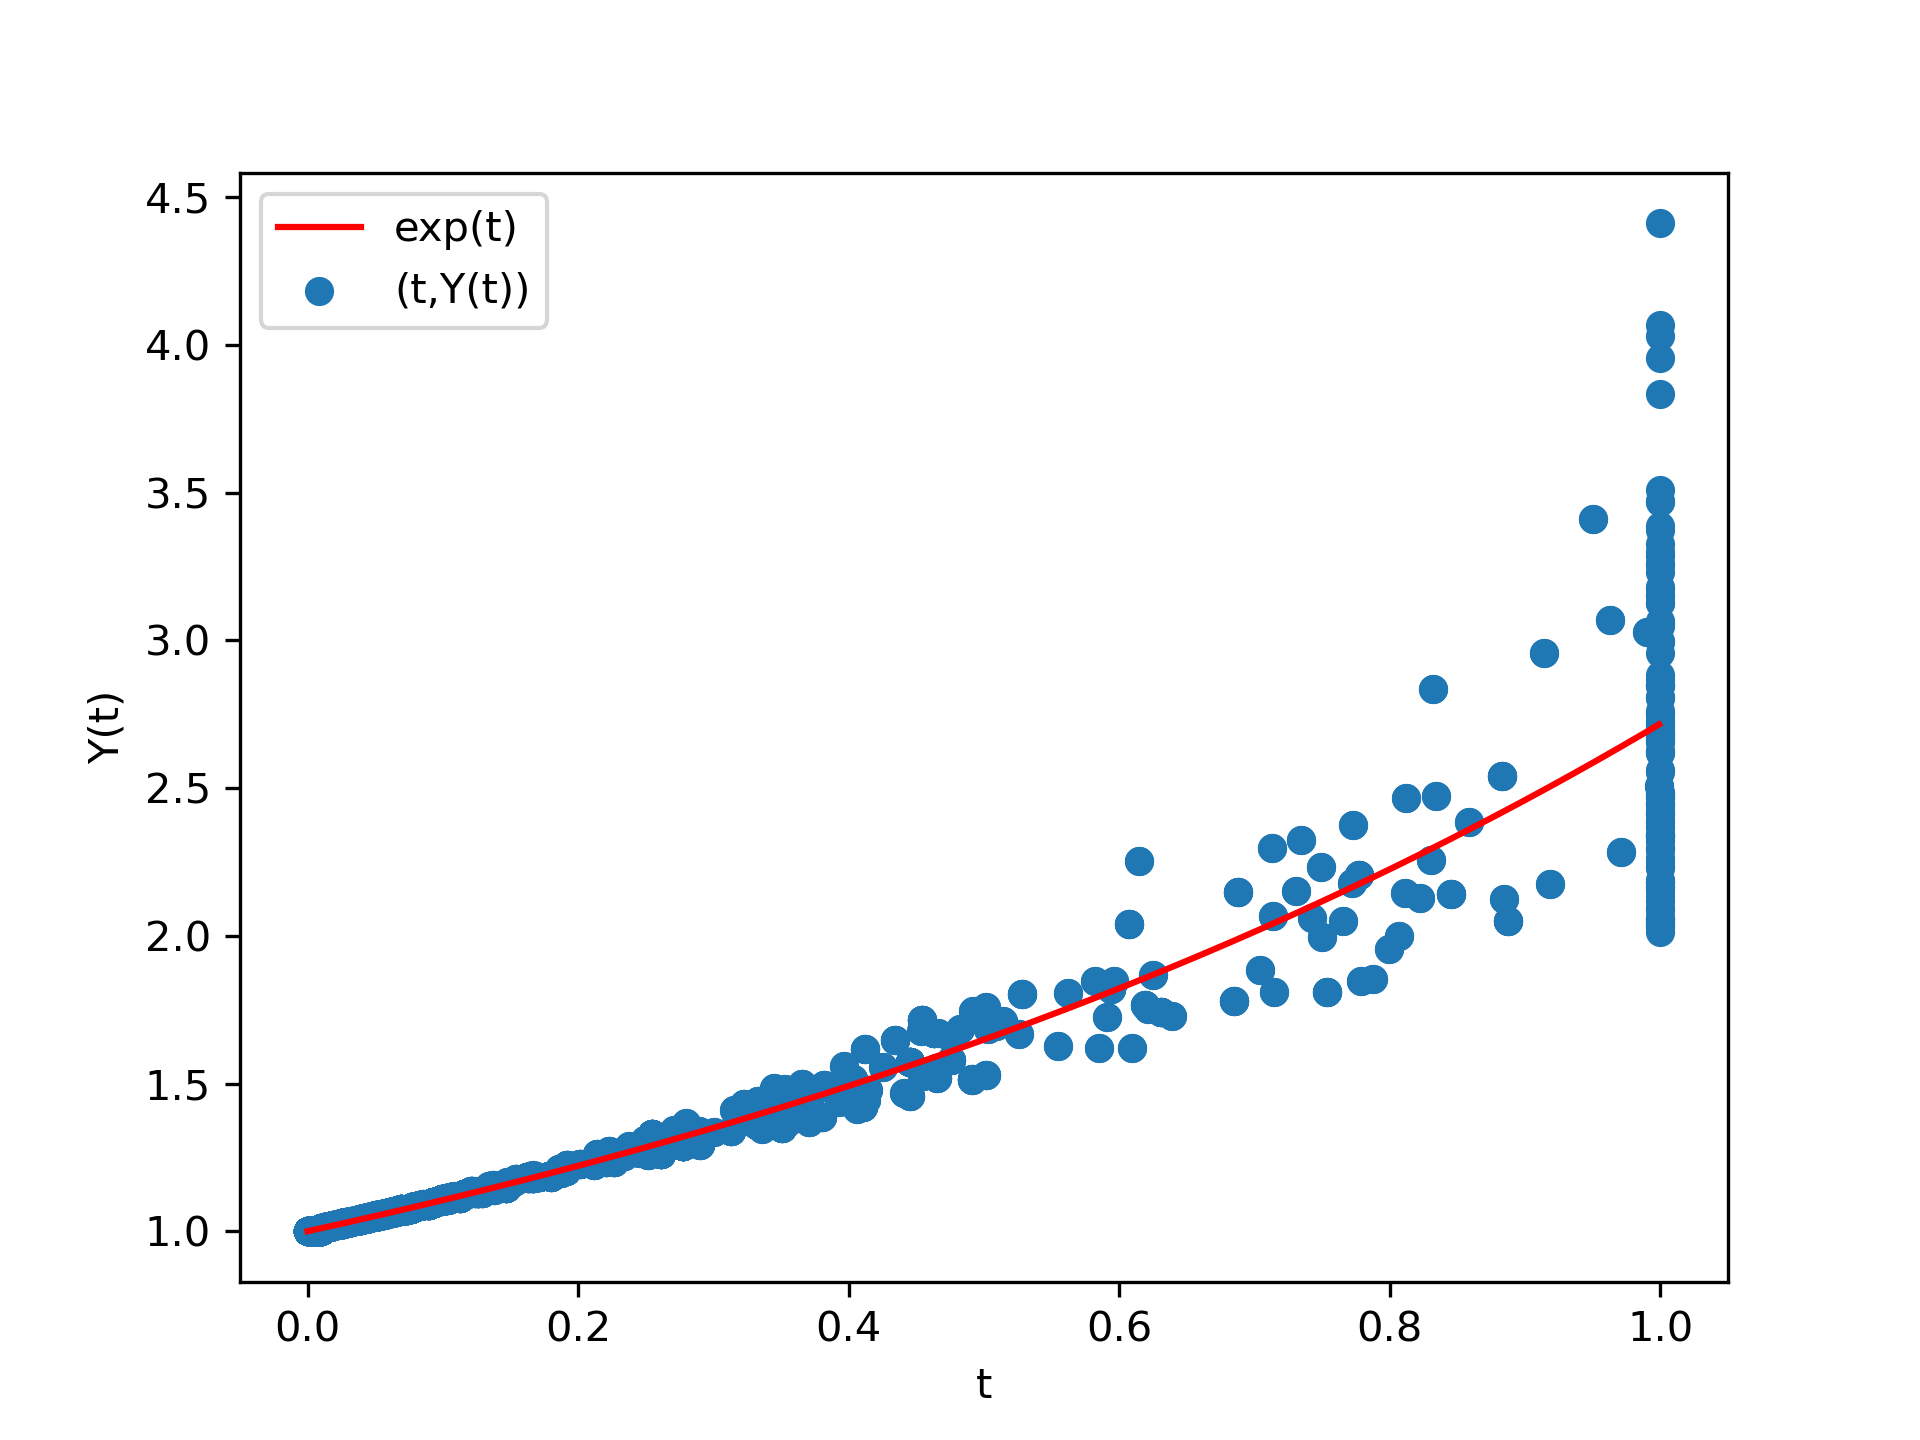
\includegraphics[width=0.8\textwidth]{plots/intro example.png}
        \caption{Recursive calls of (\ref{python eps ydy})}
        \label{fig:intro example}
    \end{figure}
\end{pythonn}

Notice that the variance of (\ref{python eps ydy})
increases rapidly as $t$ increases. This issue gets resolved
later (see (\ref{ex:RRMC IVP})).

\subsection{Modifying Monte Carlo}

In this subsection, we discuss techniques for modifying RRVEs
in a way that preserves the expected value of the solution while
acquiring more desirable properties. These techniques are only
effective when applied in a smart way by using prior information
about the problem or information about costs. \\

We will be frequently interchanging RVs with the same expectance.
That is why we introduce the following notation.
\begin{notation}[$\cong$]
    \[
        X \cong Y \iff E[X]=E[Y]
        .\]
\end{notation}

Russian roulette is a MC technique commonly employed in rendering algorithms.
The concept behind Russian roulette is to replace a RV with a
less computationally expensive approximation sometimes.

\begin{definition}[Russian roulette] \label{Russian roulette}
    We define Russian roulette on $X$ with free parameters
    $Y_{1}$, $Y_{2}$ ($E[Y_{1}] = E[Y_{2}]$), $p \in [0,1]$
    and $U$ independent of $Y_{1}$, $Y_{2}$, $X$
    as follows:

    \begin{equation}
        X \cong
        \begin{cases}
            \frac{1}{p}(X - (1-p)Y_{1}) & \text{ if } U < p \\
            Y_{2}                       & \text{ else }
        \end{cases}.
    \end{equation}
\end{definition}


\begin{notation}[$B(p)$]
    Often Russian roulette will be used with $Y_{1}= Y_{2}= 0$.
    In that case we use Bernoulli variables to shorten notation.
    \begin{equation}
        B(p) \sim \text{Bernoulli}(p) =
        \begin{cases}
            1 & \text{ if } U<p \\
            0 & \text{ else }
        \end{cases} .
    \end{equation}
\end{notation}

\begin{example}[Russian roulette] \label{ex:simple russian roulette}
    Let us consider the estimation of $E[Z]$, where $Z$ is defined as follows:

    \begin{equation}
        Z = U + \frac{f(U)}{1000}.
    \end{equation}

    Here, $f:\mathbb{R} \rightarrow [0,1]$ is an expensive function to compute.
    Directly estimating $E[Z]$ would involve evaluating $f$ in each simulation,
    which can be computationally costly. To address this, we can modify $Z$ to:

    \begin{equation}
        Z \cong U + B\left(\frac{1}{100}\right)\frac{f(U)}{10}.
    \end{equation}

    This RV requires calling $f$ on
    average once every $100$ simulations. This significantly reduces the
    computational burden while increasing the variance slightly thereby increasing
    the MC efficiency.\\
    In this  case it is also possible to estimate
    the expectance of the $2$ terms of $Z$ separately. Given the variances and
    computational complexity of both terms, you can calculate the asymptotic optimal
    division of samples for each term. But this isn't the case anymore with RMC.
\end{example}


\begin{example}[Russian roulette on (\ref{recursive RV})] \label{ex: russian roulette}
    To address the issue of indefinite recursion in equation
    (\ref{recursive RV}), Russian roulette can be employed
    by approximating the value of $Y$ near $t = 0$ with $1$
    sometimes. Specifically, we replace the coefficient $t$
    in front of the recursive term with $B(t)$ when $t < 1$.
    The modified recursive expression for $Y(t)$ becomes:

    \begin{equation}\label{eq:rr example}
        y(t) \cong Y(t) =
        \begin{cases}
            1 + B(t)Y(Ut) & \text{ if } t < 1 \\
            1 + tY(Ut)    & \text{ else}
        \end{cases}.
    \end{equation}
\end{example}

\vspace{0.2cm}

\begin{pythonn}[implementation of (\ref{eq:rr example})] \label{RRpython}
    \pythoncode{python code/RR_ydy.py}
    Interestingly, $\forall t \le 1:Y(t)$ is constrained to take on only integer values.
    This is visually clear in Figure \ref{fig:russian roulette}.
    \begin{figure}[h!]
        \centering
        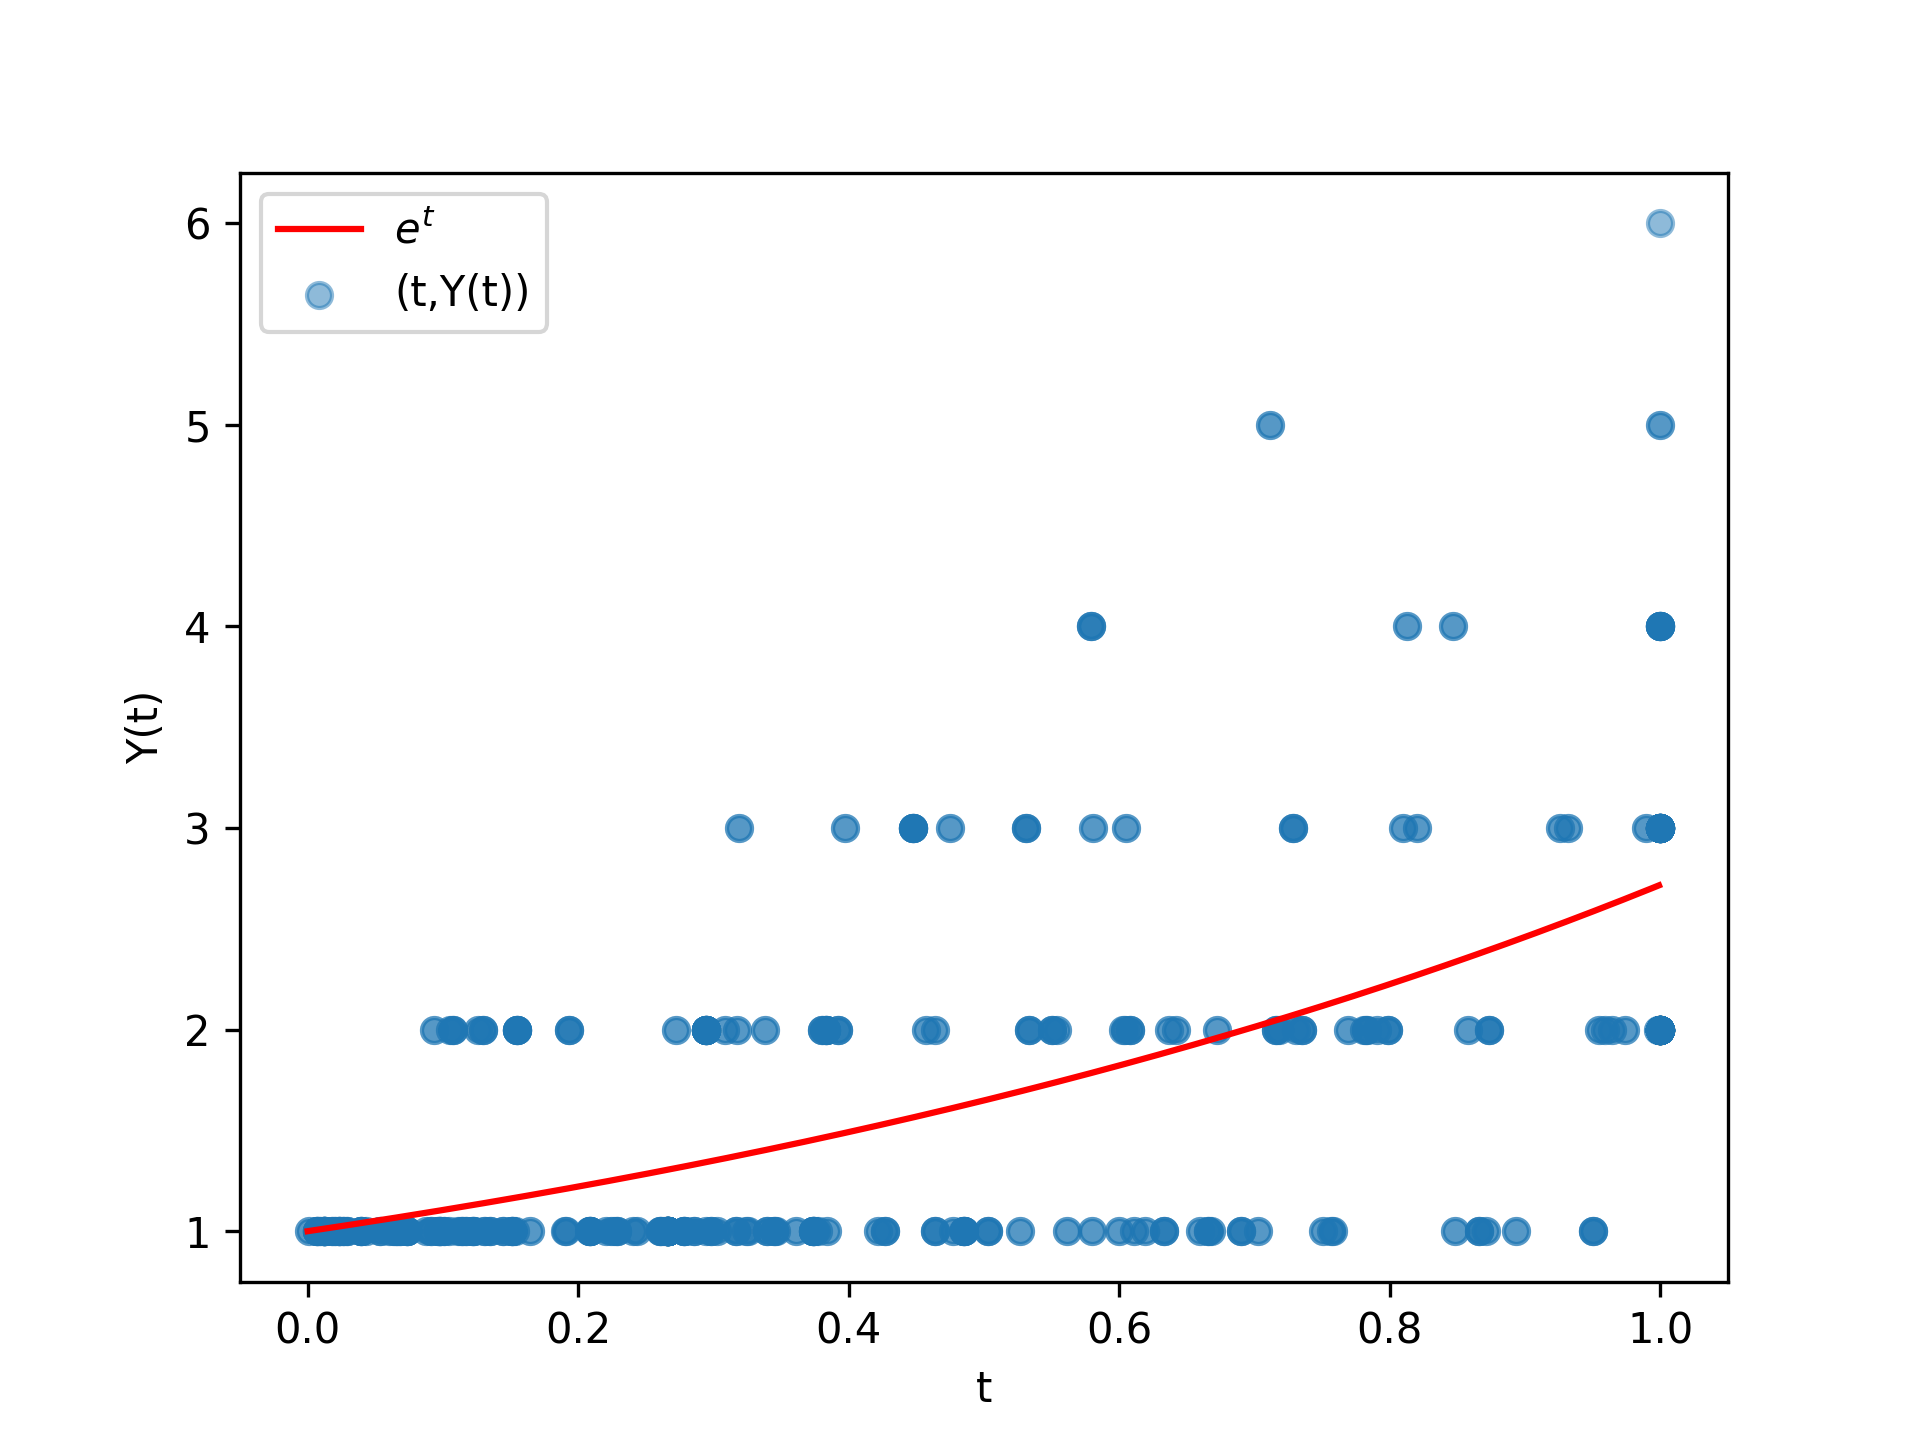
\includegraphics[width=0.8\textwidth]{plots/russian roulette example.png}
        \caption{Recursive calls $(t,Y(t))$ of (\ref{RRpython}) }
        \label{fig:russian roulette}
    \end{figure}

\end{pythonn}

Splitting is a technique that has almost the reverse effect of Russian roulette.
Instead of reducing the number of simulations of a RV as Russian roulette does,
we increase it by using more samples (i.e., splitting the sample) which
reduces the variance.

\begin{definition}[splitting] \label{def:splitting}
    Splitting $X$ refers to utilizing multiple $X_{j} \sim X$ (not necessarily independent) to
    reduce variance by taking their average:
    \begin{equation}
        X \cong \frac{1}{N} \sum_{j=1}^{N} X_{j}.
    \end{equation}
\end{definition}

Splitting the recursive term in a RRVE can result in additive branching recursion,
necessitating cautious management of terminating the branches promptly to prevent
exponential growth in computational complexity. To accomplish this, termination
strategies that have been previously discussed can be employed. Subsequently,
we will explore the utilization of coupled recursion as a technique to mitigate
additive branching recursion in RRVEs (refer to (\ref{ex:coupled splitting})).

\begin{example}[splitting on (\ref{recursive RV})] \label{ex:splitting}
    We can "split" the recursive term of Equation (\ref{recursive RV})
    into two parts as follows:

    \begin{equation}
        y(t) \cong Y(t) = 1 + \frac{t}{2}(Y_{1}(Ut) + Y_{2}(Ut)),
    \end{equation}

    where $Y_{1}(t)$ and $Y_{2}(t)$ are i.i.d. with $Y(t)$.
\end{example}

\vspace{0.2cm}

\begin{pythonn}[implementation of (\ref{ex:splitting})]
    \pythoncode{python code/SRR_ydy.py}
\end{pythonn}

\begin{definition}[control variates] \label{CV}
    Define control variating $f(X)$ with $\tilde{f}$ an approximation of $f$ as:
    \begin{equation}
        f(X) \cong (f-\tilde{f})(X) + E[\tilde{f}(X)].
    \end{equation}

    Note that control variating requires the evaluation of
    $E[\tilde{f}(X)]$. When this is estimated instead of evaluated
    exactly, we refer to it as $2$-level MC.
\end{definition}


\begin{example}[control variate on (\ref{recursive RV})] \label{ex:CV}
    To create a control variate for Equation (\ref{recursive RV}) that
    effectively reduces variance, we employ the approximation
    $y(t) \approx \tilde{y} =1+t$ and define the modified recursive term as follows:

    \begin{align}
        Y(t) & = 1 + E[\tilde{y}(Ut)] + t(Y(Ut) - \tilde{y}(Ut)) \\
             & = 1 + t + \frac{t^2}{2} + t(Y(Ut) - 1 - Ut).
    \end{align}

    It is important to note that while we could cancel out the constant term
    of the control variate, doing so would have a negative impact on
    the Russian roulette implemented later.
\end{example}

\vspace*{0.2cm}
\begin{pythonn}[implementation of (\ref{ex:CV})]
    \pythoncode{python code/CVRR_ydy.py}
\end{pythonn}

\begin{related}[MC modification]
    For further reference on these techniques see \cite{veach_robust_1997}.
\end{related}

\subsection{Monte Carlo Trapezoidal Rule}

In this subsection, we introduce a MC trapezoidal rule that
exhibits similar convergence behavior to the methods discussed later.
The MC trapezoidal rule is essentially a regular Monte Carlo method
enhanced with control variates based on the trapezoidal rule.

\begin{definition}[MC trapezoidal rule]
    We define the MC trapezoidal rule for approximating the integral
    of function $f$ over the interval $[x, x+\Delta x]$ with a Russian roulette rate
    $l$ and $\tilde{f}$ the linear approximation of $f$ corresponding
    to the trapezoidal rule as follows:

    \begin{align}
         & \int_{x}^{x+\Delta x} f(s) ds                           \\
         & = \int_{x}^{x+\Delta x}  \tilde{f}(s) ds +
        \int_{x}^{x+\Delta x}  f(s) - \tilde{f}(s) ds              \\
         & = \Delta x \frac{f(x) + f(x+\Delta x)}{2}
        + E \left[f(S) - \tilde{f}(S)\right]                       \\
         & \cong \Delta x \frac{f(x) + f(x+\Delta x)}{2} \nonumber \\
         & + \Delta x l B\left( \frac{1}{l}\right)
        \left(f(S) - f(x) - \frac{S - x}{\Delta x}
        \left(f(x+\Delta x) - f(x)\right) \right), \label{eq:MCtrap}
    \end{align}

    where $S \sim \text{Uniform}(x,x+\Delta x)$.
\end{definition}

\begin{lemma}[RMSE MC Trapezoidal Rule] \label{lem:rmse mctrap}
    The MC trapezoidal rule
    for a twice differentiable function has
    \begin{equation}
        \text{RMSE} =O\left( \Delta x^{3} \right) .
    \end{equation}
\end{lemma}

\begin{proof}
    Start from equation (\ref{eq:MCtrap}). The MSE is the variance
    so we can ignore addition by constants.

    \begin{equation}
        \text{MSE} = \text{Var}\left( \Delta x l B\left( \frac{1}{l}\right)
        \left(f(S) - f(x) - \frac{S - x}{\Delta x}
        \left(f(x+\Delta x) - f(x)\right) \right)\right)
    \end{equation}
    We substitute $S = \Delta x U + x$ and then apply Taylor's theorem
    finishing the proof:

    \begin{align}
        \text{MSE} & = \text{Var}\left( \Delta x l B\left( \frac{1}{l}\right)
        \left(f(xU+x) - f(x) - U
        \left(f(x+\Delta x) - f(x)\right) \right)\right)                           \\
                   & = \text{Var}\left( \Delta x l B\left( \frac{1}{l}\right)
        \left( U \Delta x f'(x)+ \frac{U^{2} \Delta x ^{2}}{2} f''(Z_{1})
        - U \left( \Delta x f'(x) +
        \Delta x ^{2} f''(z_{2})\right) \right)\right)                             \\
                   & = \text{Var}\left( \Delta x l B\left( \frac{1}{l}\right)
        \left( \frac{U^{2} \Delta x ^{2}}{2} f''(Z_{1})
        -  \frac{U\Delta x ^{2}}{2} f''(z_{2}) \right)\right)                      \\
                   & =\Delta x ^{6} \text{Var}\left(  l B\left( \frac{1}{l}\right)
        \left( \frac{U^{2} }{2} f''(Z_{1})
        -  \frac{U}{2} f''(z_{2}) \right)\right),
    \end{align}
    for some $Z_{1} \in [x,S], z_{2} \in [x,x+\Delta x]$.
\end{proof}
Note that the proof doesn't rely on Russian roulette ($l=1$).


\begin{definition}[composite MC trapezoidal rule] \label{MCtrap}
    Define the composite MC trapezoidal rule for approximating the integral
    of function $f$ over the interval $[a, b]$ for a uniform grid $(x_{j})$ with $n$
    intervals and a Russian roulette rate $l$ as follows:

    \begin{align} \label{eq:cMCtrap}
        \int_{a}^{b} f(s) ds \cong \Delta x \sum_{j=1}^{n} & \frac{f(x_{j}) + f(x_{j}+\Delta x)}{2} \nonumber \\
                                                           & + l B\left(\frac{1}{l}\right)
        \left(f(S_j) - f(x_{j}) - \frac{S_j - x_{j}}{\Delta x}(f(x_{j}+\Delta x) - f(x_{j}))\right),
    \end{align}

    where $S_j \sim \text{Uniform}(x,x+\Delta x)$.

\end{definition}

\begin{pythonn}[implementation of (\ref{MCtrap})]
    We implement (\ref{MCtrap}) for $\int_{0}^{1}e^{s}ds$.
    \vspace*{0.5cm}
    \pythoncode{python code/trap1.py}

    \begin{figure}[h!]
        \centering
        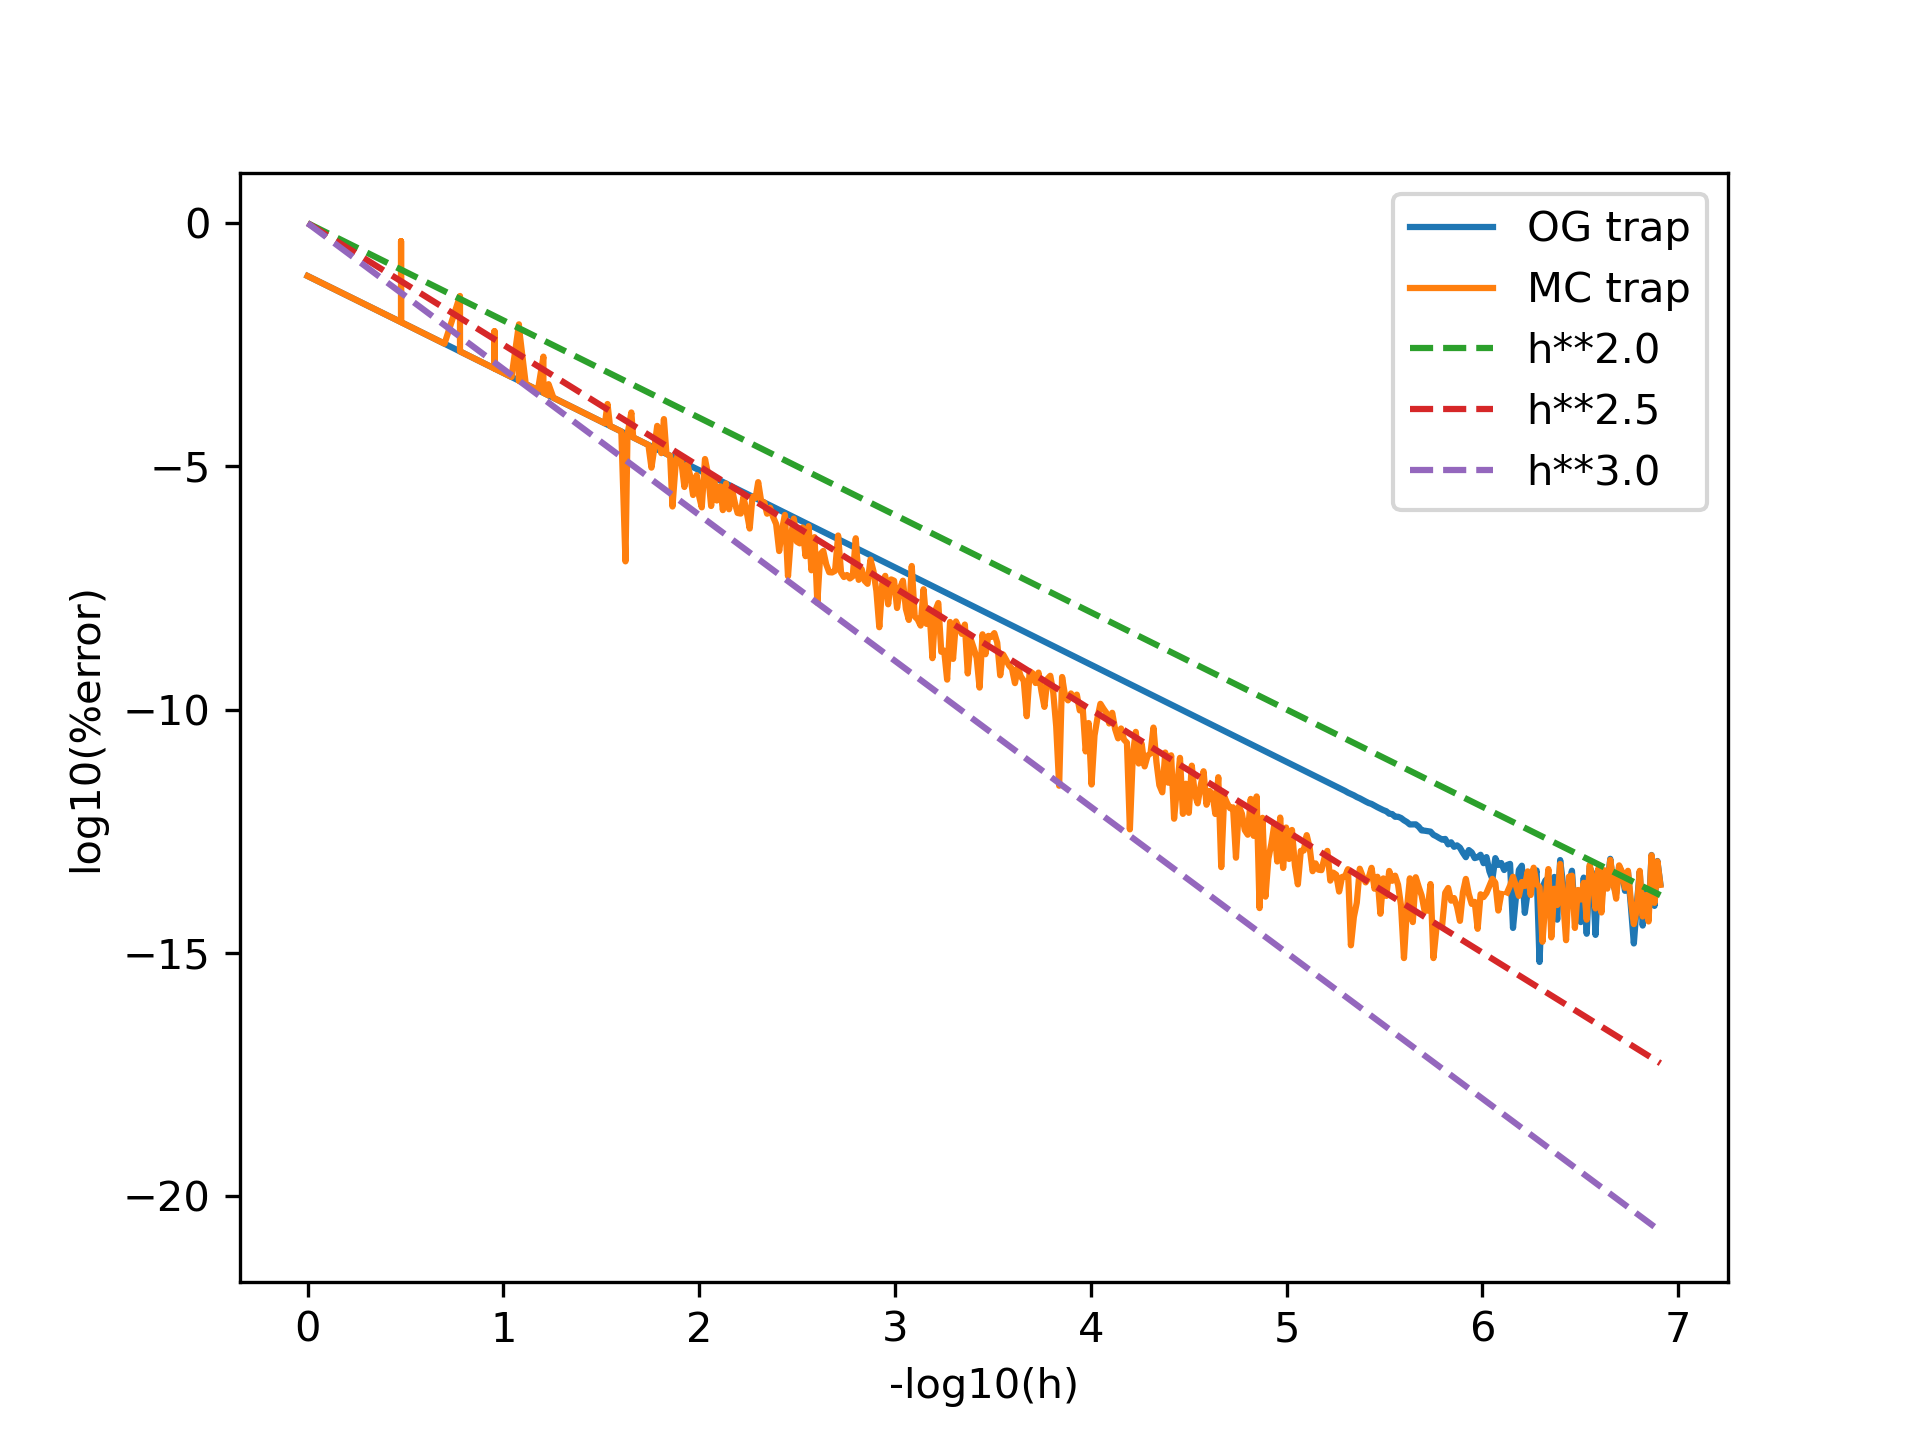
\includegraphics[width=0.8\textwidth]{plots/MCtrap.png}
        \caption{Log-log plot of the error of (\ref{MCtrap}) for
        $\int_{0}^{1}e^{s}ds$ with $l=100$. At floating point accuracy,
        the convergence ceases.
        }
        \label{fig:MCtrap}
    \end{figure}
\end{pythonn}

Figure \ref{fig:MCtrap} suggest that the order of convergence of RMSE of the
MC trapezoidal rule is better by $0.5$ as the normal trapezoidal rule.
The MC trapezoidal rule has on average $\frac{1}{l}$ more function calls than
the normal trapezoidal rule. For the composite rule with $n$ intervals,
there are $\text{Binomial}(n,\frac{1}{l})$ additional function calls
(repeated Bernoulli experiments). So they use up to a constant the same amount
of function calls. This implies an advantage in IBC. \\

\begin{theorem}[RMSE Composite Trapezoidal MC Rule] \label{thrm:order trap}
    The composite trapezoidal MC rule  wth $n$ intervals
    for a twice differentiable function has
    \begin{equation}
        \text{RMSE} =O\left(\frac{1}{n^{2.5}} \right) .
    \end{equation}

\end{theorem}

The proof uses lemma \ref{lem:rmse mctrap}
and is similar to the proof of the normal
trapezoidal rule with the main difference being  the
accumulation of ''local truncation'' errors into ''global truncation'' error.
Normally there is a loss of one order but the MC trapezoidal loses only a half order
because the accumulation happens in variance instead of bias.

\begin{align}
    \sqrt{\text{Var}\left(\sum_{j=1}^{n} h^{3}U_{j}^{2}\right)}
     & =h^{3} \sqrt{ \sum_{j=1}^{n}\text{Var} (U_{j}^{2})} \\
     & =h^{3} \sqrt{ n \text{Var}(U^{2})}                  \\
     & = O(h^{2.5}).
\end{align}

Note that the meaning of a bound on the error that behaves as $O(h^{2})$ and
a bound on the RMSE that behaves as $O(h^{2})$ is different.
A bound on the error implies a bound on the RMSE, but
the reverse is not true.

\begin{related}[Monte Carlo Trapezoidal Rule]
    With Stein's paradox it is always possible to bias the composite MC trapezoidal
    rule to achieve lower RMSE.
    The optimal IBC for RMSE for some smoothness classes
    are known see \cite{heinrich_optimal_2001}.
\end{related}


\subsection{Unbiased Non-Linearity}

In this subsection, we present techniques for handling polynomial non-linearity.
The backbone for this is using independent samples
$y^{2} \cong Y_{1} Y_{2}$ with $Y_{1}$ independent of $ Y_{2}$ and
$Y_{1} \cong Y_{2} \cong y$.


\begin{example}[$y'=y^{2}$] \label{ex:nonlinear example}
    Consider the following ODE:

    \begin{equation} \label{eq:nonlinear example}
        y' = y^2, \quad y(1) = -1.
    \end{equation}

    The solution to this equation is given by $y(t) = -\frac{1}{t}$.
    By integrating both sides of equation (\ref{eq:nonlinear example}),
    we obtain the following integral equation:

    \begin{equation}
        y(t) = -1 + \int_{1}^{t} y(s) y(s)ds.
    \end{equation}

    To estimate the recursive integral in equation (\ref{eq:nonlinear example}),
    we use i.i.d. $Y_1,Y_2 \sim Y$ in following RRVE:

    \begin{equation} \label{RRVE: nonlinear example}
        y(t) \cong Y(t) = -1 + (t-1) Y_1(S) Y_2(S),
    \end{equation}

    where $S \sim \text{Uniform}(1,t)$.
    Branching RRVEs are typical when dealing
    with non-linearity.
\end{example}

\vspace*{0.2cm}
\begin{pythonn}[implementation (\ref{ex:nonlinear example})]\label{py:nonlinear example}
    \pythoncode{python code/dyy2.py}
    In this implementation $Y(t)$ only takes values $\{-1,0\}$.
\end{pythonn}

\begin{example}[$e^{E[X]}$] \label{ex:exp int}
    $e^{\int x(s)ds}$ is a common expression encountered when studying ODEs.
    In this example, we demonstrate how you can generate unbiased estimates of
    $e^{E[X]}$ with simulations of $X$. The Taylor series of $e^{x}$ is:
    \begin{align}
        e^{E[X]} & = \sum_{n=0}^{\infty} \frac{E^{n}[X]}{n!}     \\
                 & = 1 + \frac{1}{1}E[X]\left(1+ \frac{1}{2}E[X]
        \left(1+\frac{1}{3}E[X]\left(1+ ...\right)\right)\right). \label{taylor e}
    \end{align}
    Change the fractions of equation (\ref{taylor e}) to Bernoulli processes
    and replace all $X$ with independent $X_j$ with $E[X]=E[X_{i}]$.
    \begin{align}
        e^{E[X]} & = E
        \left[1 + B\left(\frac{1}{1}\right)E[X_1]
        \left(1+ B\left(\frac{1}{2}\right)E[X_2]
        \left(1+B\left(\frac{1}{3}\right)E[X_3]
        \left(1+ ...\right)
        \right)
        \right)
        \right]              \\
                 & = E\left[
            1 + B\left(\frac{1}{1}\right)X_1
            \left(1+ B\left(\frac{1}{2}\right)X_2
            \left(1+B\left(\frac{1}{3}\right)X_3
            \left(1+ ...\right)
            \right)
            \right)
            \right]
    \end{align}
    What is inside the expectation is something that we can simulate with simulations of $X_{j}$.
\end{example}

\begin{related}[example \ref{ex:exp int}]
    NVIDIA has a great paper on optimizing example \ref{ex:exp int}
    \cite{kettunen_unbiased_2021}.
\end{related}

\subsection{Recursion}

In this subsection, we discuss recursion-related techniques.

\begin{technique}[coupled recursion]
    The idea behind coupled recursion is sharing recursion calls of
    multiple RRVEs for simulation. This does make them dependent.
\end{technique}

\begin{example}[coupled recursion] \label{ex:coupled recursion}
    Consider calculating the
    sensitivity of following ODE to a
    parameter $a$:
    \begin{align}
        y'             & =ay,y(0)=1 \Rightarrow \label{couple recu ex1} \\
        \partial_{a}y' & = y + a \partial_{a}y \label{couple recu ex2}
    \end{align}
    Turn (\ref{couple recu ex1}) and (\ref{couple recu ex2}) into RRVEs.
    To emphasize that they are coupled, that they should
    recurse together we write them in a matrix equation:
    \begin{equation} \label{coupled mat}
        \begin{bmatrix}
            Y(t) \\
            \partial_{a}Y(t)
        \end{bmatrix}=
        X(t)=
        \begin{bmatrix}
            1 \\
            0
        \end{bmatrix}+
        t \begin{bmatrix}
            a & 0 \\
            1 & a
        \end{bmatrix}
        X(Ut).
    \end{equation}

    Observe how this eliminates the additive branching recursion
    present in equation (\ref{couple recu ex2}).

\end{example}

\begin{pythonn} [implementation of (\ref{coupled mat})]
    \pythoncode{python code/coupled_mat.py}
\end{pythonn}

\begin{related}[coupled recursion]
    Example \ref{ex:coupled recursion} is inspired by \cite{vicini_path_2021}.
    \cite{vicini_path_2021} propose an efficient unbiased backpropagation
    algorithm for rendering.
\end{related}

\begin{technique}[recursion in recursion]\label{tech:recu in recu}
    Recursion in recursion is like proving an induction
    step of an induction proof with induction. Recursion in recursion
    uses an inner recursion in the outer recursion.
\end{technique}

\begin{related}[recursion in recursion]
    Beautiful examples of recursion in recursion are
    the next flight variant of WoS in
    \cite{sawhney_grid-free_2022} and epoch-based algorithms in optimization
    \cite{gupta_convergence_2021}.
\end{related}

Most programming languages do support recursion, but it often comes with certain
limitations such as maximum recursion depth and potential performance issues.
There are multiple ways to implement recursion we will discuss tail recursion and
do an example using a stack.

\begin{technique}[non-branching tail recursion]
    Tail recursion involves reordering all operations
    so that almost no operation needs to happen after
    the recursion call. This allows us to return the
    answer without retracing all steps when we reach
    the last recursion call and it can achieve similar
    speeds to a forward implementation.
\end{technique}

The non-branching recursion presented in the RRVEs
can be implemented with tail recursion due to the associativity of
all operations ($(xy)z = x(yz)$) involved.

\begin{pythonn}[tail recursion on (\ref{coupled mat})] \label{py:tail recursion couple}
    We implement (\ref{coupled mat}) but this time with tail recursion.
    We collect addition operations in a vector $sol$ and multiplication
    in a matrix $W$. $W$ may be referred to as accumulated weight or throughput.
    \vspace{0.3cm}
    \pythoncode{python code/tailrecu.py}
\end{pythonn}

Tail recursion is not always desirable as it discards intermediate values of
the recursion calls and can increase
computational cost.
To retain some of these intermediate values, it is possible to use tail recursion partially.
In example \ref{py:tail recursion couple} it would
be more efficient to avoid matrix multiplication on line $7$. An alternative
to tail recursion is implementing the recursion with a stack.

\begin{pythonn}[stack recursion on (\ref{coupled mat})] \label{py:stack recursion couple}
    We implement (\ref{coupled mat}) but this time with a stack.
    We want to avoid matrix multiplication and only use matrix-vector multiplications.
    To do this on (\ref{coupled mat}) we need to know $X(Ut)$ when
    it doesn't get Russian rouletted away. If we sample $Ut$ we can recurse
    on our reasoning until Russian roulette termination so we need the path
    of all the samples.
    \vspace{0.3cm}
    \pythoncode{python code/stackrecu.py}
\end{pythonn}


\section{Ordinary Differential Equations}

\subsection{Green Functions}
In this subsection, we discuss informally how to turn ODEs into integral equations mainly
by example. Our main tool for this are green functions.
Prior to discussing green functions, we offer several
examples.

\begin{notation}[$H$]
    We denote the Heaviside step function with:
    \begin{equation}
        H(x) = \begin{cases}
            0 & \text{ if } x<0 \\
            1 & \text{ else }
        \end{cases}.
    \end{equation}
\end{notation}

\begin{example}[$y'=y$ average condition]
    We will solve the equation:

    \begin{equation} \label{ydy int}
        y' = y,
    \end{equation}

    but this time with a different condition:

    \begin{equation}
        \int_{0}^{1} y(s) ds = e-1.
    \end{equation}

    The solution to this equation remains the same: $y(t) = e^{t}$.
    We define the corresponding source green function $G(t,x)$ for $y'$
    and this type of condition as follows:

    \begin{equation}
        G' = \delta(x-t), \quad \int_{0}^{1} G(s,x) ds = 0.
    \end{equation}

    Solving this equation yields:

    \begin{equation}
        G(t,x) = H(t-x) + x - 1.
    \end{equation}

    It is worth noting that we could have chosen a different
    green function corresponding to a different linear
    differential operator.

    At this point, it may not be clear, but using this green function,
    we can form the following integral equation for (\ref{ydy int}):

    \begin{equation} \label{int ydy int}
        y(t) = e - 1 + \int_{0}^{1} G(t,s) y(s) ds.
    \end{equation}

    Converting equation (\ref{int ydy int}) into a RRVE
    using RMC, we obtain:

    \begin{equation}\label{RRVE ydy int}
        Y(t) = e - 1 + 2B\left(\frac{1}{2}\right)Y(S)(H(t-S)+S-1),
    \end{equation}

    where $S \sim U$. We will skip the Python implementation
    of equation (\ref{RRVE ydy int}) as it does not provide any
    new information. Instead, we will plot realizations of
    equation (\ref{RRVE ydy int}) in Figure \ref{fig:ydy int}.

    \begin{figure}[h!]
        \centering
        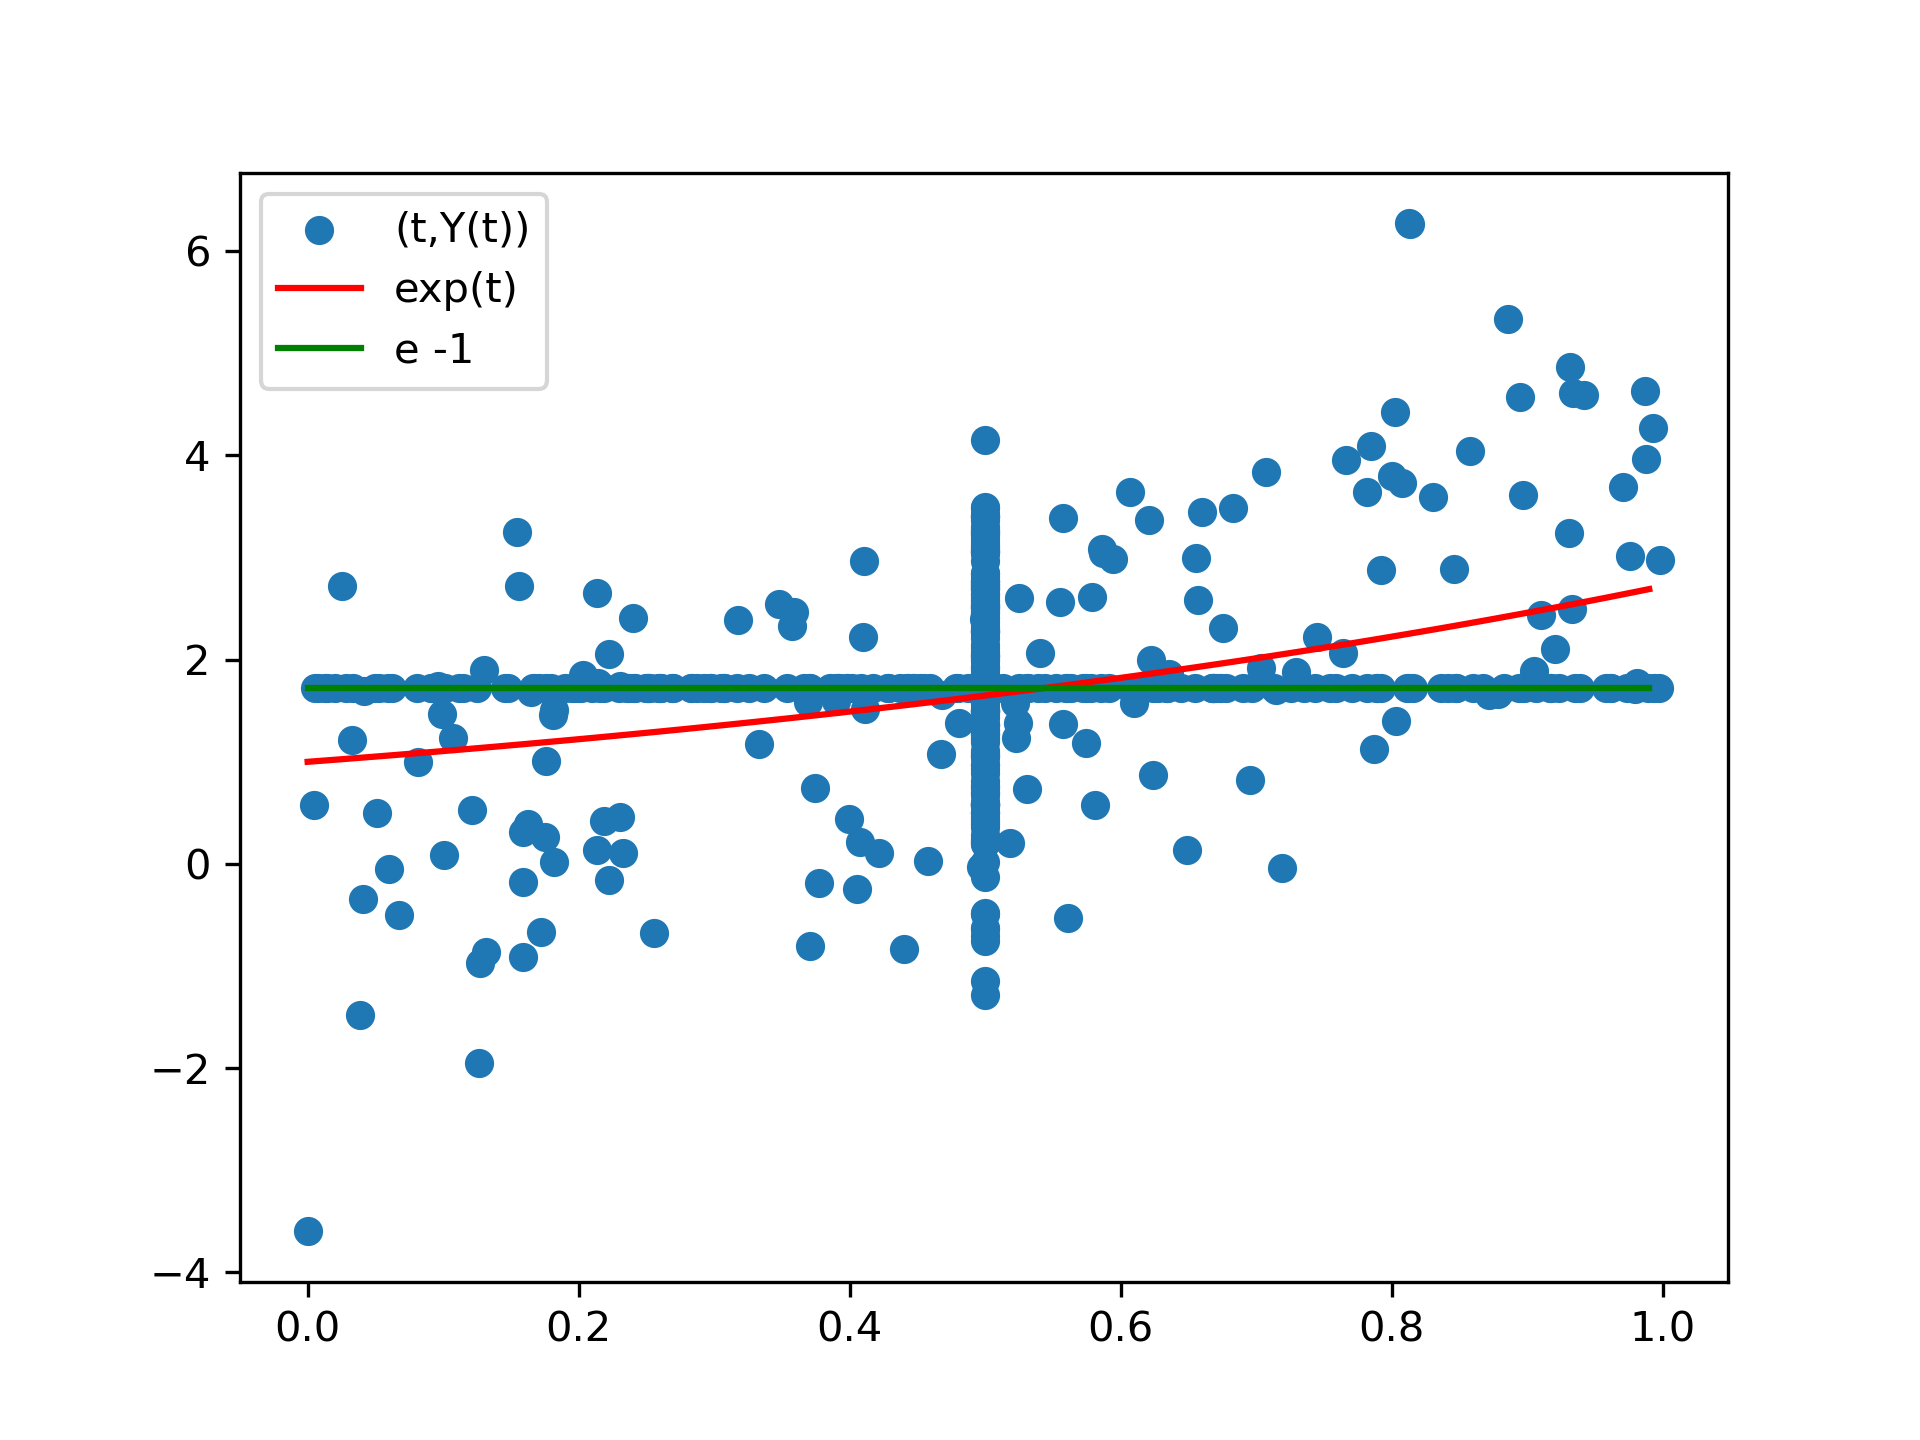
\includegraphics[width=0.8\textwidth]{plots/ydy int.png}
        \caption{Recursive calls of (\ref{RRVE ydy int}) when
            calling $Y(0.5)$ $300$ times. Points accumulate on
            the green line due to the Russian roulette,
            and at  $t=0.5$ because it is the starting
            value of the simulation.
        }
        \label{fig:ydy int}
    \end{figure}

\end{example}

% Green's function vs green function (check chatgpt for the answer)
\begin{definition}[green function]
    Vaguely speaking, we define the green function as a type
    of kernel function used to solve linear problems with linear
    conditions. The green function is the kernel that we
    place in front of the linear conditions or the source term,
    which we integrate over to obtain the solution. The green
    function possesses the property of satisfying either null
    linear conditions and a Dirac delta source term, or vice versa.
\end{definition}

\begin{related}[green function]
    Our notion of green function is similar to that in \cite{hwang_simulationtabulation_2001}.
\end{related}

% maybe an example of difference equation

% \subsection{Convergence}
\subsection{Fredholm Integral Equations}

\textcolor{green}{
    TODO:
    \begin{itemize}
        \item explain better the graph for coupled splitting
        \item add better explaination to coupled splitting
    \end{itemize}
}

The integral equations obtained in the previous subsection are Fredholm integral
equations of the second kind. In this subsection, we introduce a technique called
coupled splitting.


\begin{definition}[Fredholm equation of the second kind]
    A Fredholm equation of the second kind for $\varphi$  is of the following form:
    \begin{equation}
        \varphi(t)=f(t)+\lambda \int_a^b K(t, s) \varphi(s) ds.
    \end{equation}
    Given the kernel  $K(t, s)$  and  $ f(t)$.
\end{definition}

If both $K$ and $f$ satisfy certain regularity conditions, then for sufficiently
small $\lambda$, it is relatively straightforward to establish the existence
and uniqueness of solutions using a fixed-point argument.

% We would like to have MC algorithm that converges in that case. Our best guess is
% a combination of splitting and coupling.

\begin{example}[Dirichlet $y''=y$] \label{main dirichlet}
    The following ODE will be the main testing example for
    boundary value problems:
    \begin{equation} \label{eq:main dirichlet}
        y''=y, \quad y(b_{0}),y(b_{1}).
    \end{equation}
    The green functions corresponding to $y''$ and Dirichlet conditions are:

    \begin{align}
        P(t,x) & = \begin{cases}
                       \frac{b_{1}-t}{b_{1}-b_{0}} & \text{if } x = b_{0} \\
                       \frac{t-b_{0}}{b_{1}-b_{0}} & \text{if } x = b_{1}
                   \end{cases},       \\
        G(t,s) & = \begin{cases}
                       -\frac{(b_{1}-t)(s-b_{0})}{b_{1}-b_{0}} & \text{if } s<t \\
                       -\frac{(b_{1}-s)(t-b_{0})}{b_{1}-b_{0}} & \text{if } t<s
                   \end{cases}.
    \end{align}
    Straight from these green functions you get the following integral equation and RRVE:
    \begin{align} \label{inteq:main dirichlet}
        y(t) & = P(t,b_{0}) y(b_{0}) + P(t,b_{1}) y(b_{1}) +
        \int_{b_{0}}^{b_{1}} G(t,s)y(s) ds,                  \\
        Y(t) & = P(t,b_{0}) y(b_{0}) + P(t,b_{1}) y(b_{1})
        + l B\left(\frac{1}{l} \right)(b_{1}-b_{0}) G(t,S)y(S) , \label{RRVE:main dirichlet}
    \end{align}
    where $l \in \mathbb{R}$ the Russian roulette rate is and
    $S \sim \text{Uniform}(b_{1},b_{0})$.

\end{example}


\begin{example}[coupled splitting on (\ref{main dirichlet})] \label{ex:coupled splitting}
    In addition to normal splitting (see Definition \ref{def:splitting}),
    we can also split the domain in Equation (\ref{inteq:main dirichlet})
    as follows:

    \begin{align}\label{inteq:coupled splitting}
        y(t) & = P(t,b_{0}) y(b_{0}) + P(t,b_{1}) y(b_{1}) +
        \frac{1}{2} \int_{b_{0}}^{b_{1}} G(t,s)y(s) ds +
        \frac{1}{2} \int_{b_{0}}^{b_{1}} G(t,s)y(s) ds,                                             \\
        y(t) & = P(t,b_{0}) y(b_{0}) + P(t,b_{1}) y(b_{1}) + \label{inteq:coupled domain splitting}
        \int_{b_{0}}^{\frac{b_{1}+b_{0}}{2}} G(t,s)y(s) ds +
        \int_{\frac{b_{1}+b_{0}}{2}}^{b_{1}} G(t,s)y(s) ds.
    \end{align}

    By coupling, we can eliminate the additive branching recursion
    in the RRVEs corresponding to Equations (\ref{inteq:coupled splitting})
    and (\ref{inteq:coupled domain splitting}).
    This results in the following RRVE:

    \begin{equation} \label{RRVE:coupled splitting}
        X(t_{1},t_{2})=
        \begin{bmatrix}
            P(t_{1},b_{0}) & P(t_{1},b_{1}) \\
            P(t_{2},b_{0}) & P(t_{2},b_{1})
        \end{bmatrix}
        \begin{bmatrix}
            y(b_{0}) \\
            y(b_{1})
        \end{bmatrix}
        +
        W
        \begin{bmatrix}
            G(t_{1},S_{1}) & G(t_{1},S_{2}) \\
            G(t_{2},S_{1}) & G(t_{2},S_{2})
        \end{bmatrix}
        X(S_{1},S_{2}),
    \end{equation}
    where $W$ the right weighting matrix is
    (see code (\ref{py:coupled splitting})),
    and $S_{1}$ and $S_{2}$ can be chosen
    in various ways.
\end{example}

\begin{pythonn}[implementation of (\ref{RRVE:coupled splitting})] \label{py:coupled splitting}
    We implemented equation (\ref{RRVE:coupled splitting}) in example
    (\ref{ex:coupled splitting}) with recursion but in this case, it
    is also possible to implement it forwardly. \\
    \pythoncode{python code/coupled_splitting.py}

    % can probably make a better plot then this one
    \begin{figure}[h!]
        \centering
        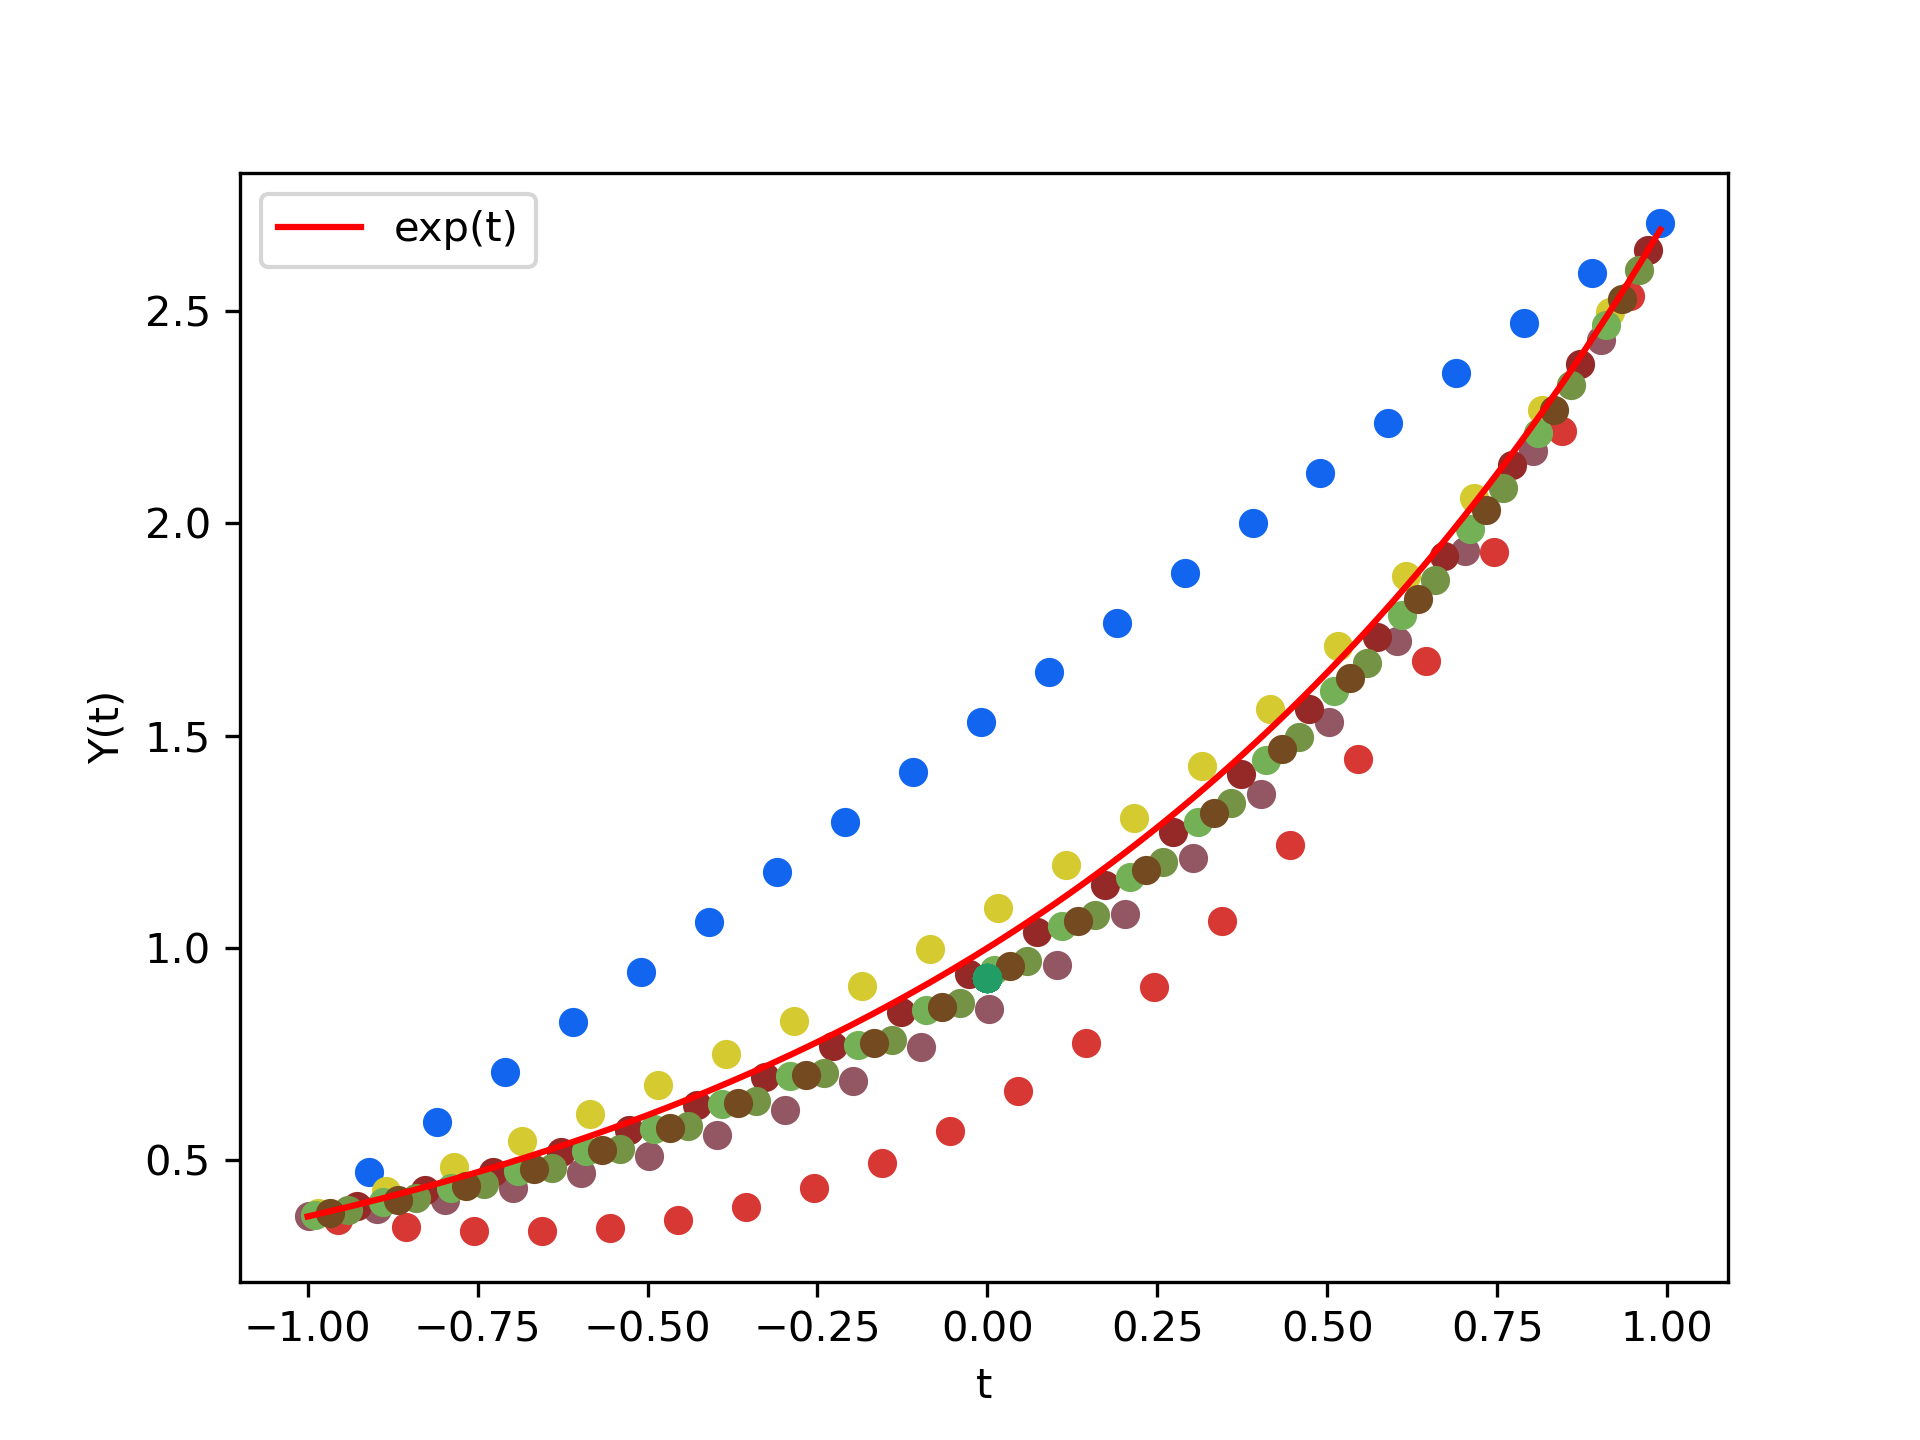
\includegraphics[width=0.8\textwidth]{plots/coupled split.png}
        \caption{Recursive calls of equation (\ref{RRVE:coupled splitting}) when
        calling $X(0)$ once,
        with a split size of $20$, $S_{j}$ are coupled such
        they are equally spaced and the coupling is colored.
        The initial conditions for this call are $y(-1)=e^{-1}$ and $y(1)=e^{1}$,
        with Russian roulette rate $l=1.2$.  }
        \label{fig:coupled splitting}
    \end{figure}
\end{pythonn}


Example (\ref{ex:coupled splitting}) does not
exploit the locality and smoothness of the problem.
We conjecture that coupled splitting can be particularly valuable when
dealing with linear Fredholm equations of the second kind,
especially in scenarios where MC integration surpasses
traditional integration methods. This holds true for
high-dimensional problems, non-smooth kernels, and
challenging domains. We conjecture that employing
coupled splitting in such cases can yield favorable results.

\begin{related}[coupled splitting]
    Coupled splitting is partly inspired by how \cite{sabelfeld_sparsified_2009}
    reduces variance by using bigger submatrices.
    Reusing samples for walk on sphere gets discussed
    in \cite{miller_boundary_2023} and \cite{bakbouk_mean_2023}.
\end{related}

Figure \ref{fig:coupled splitting}
resembles fixed-point iterations, leading us to hypothesize
that coupled splitting can achieve convergence in most cases
where a fixed-point argument holds true and the convergence
speed is very similar to fix-points methods until the accuracy
of the stochastic approximation of the operator is reached
(the approximate operator bottleneck). The approximation of the operator
can be improved by increasing coupled splitting amount when
approaching the bottleneck. Alternatively when reaching
the bottleneck it is possible to rely on MC convergence.

\begin{related}[convergence coupled splitting]
    See \cite{gupta_convergence_2021} for a discussion on the convergence
    of recursive stochastic algorithms.
\end{related}

Coupled splitting was originally motivated to help with
convergence. It didn't increase the convergence domain for
the example shown in Figure \ref{fig:mainD explosion}.\\

\begin{figure}[h!]
    \centering
    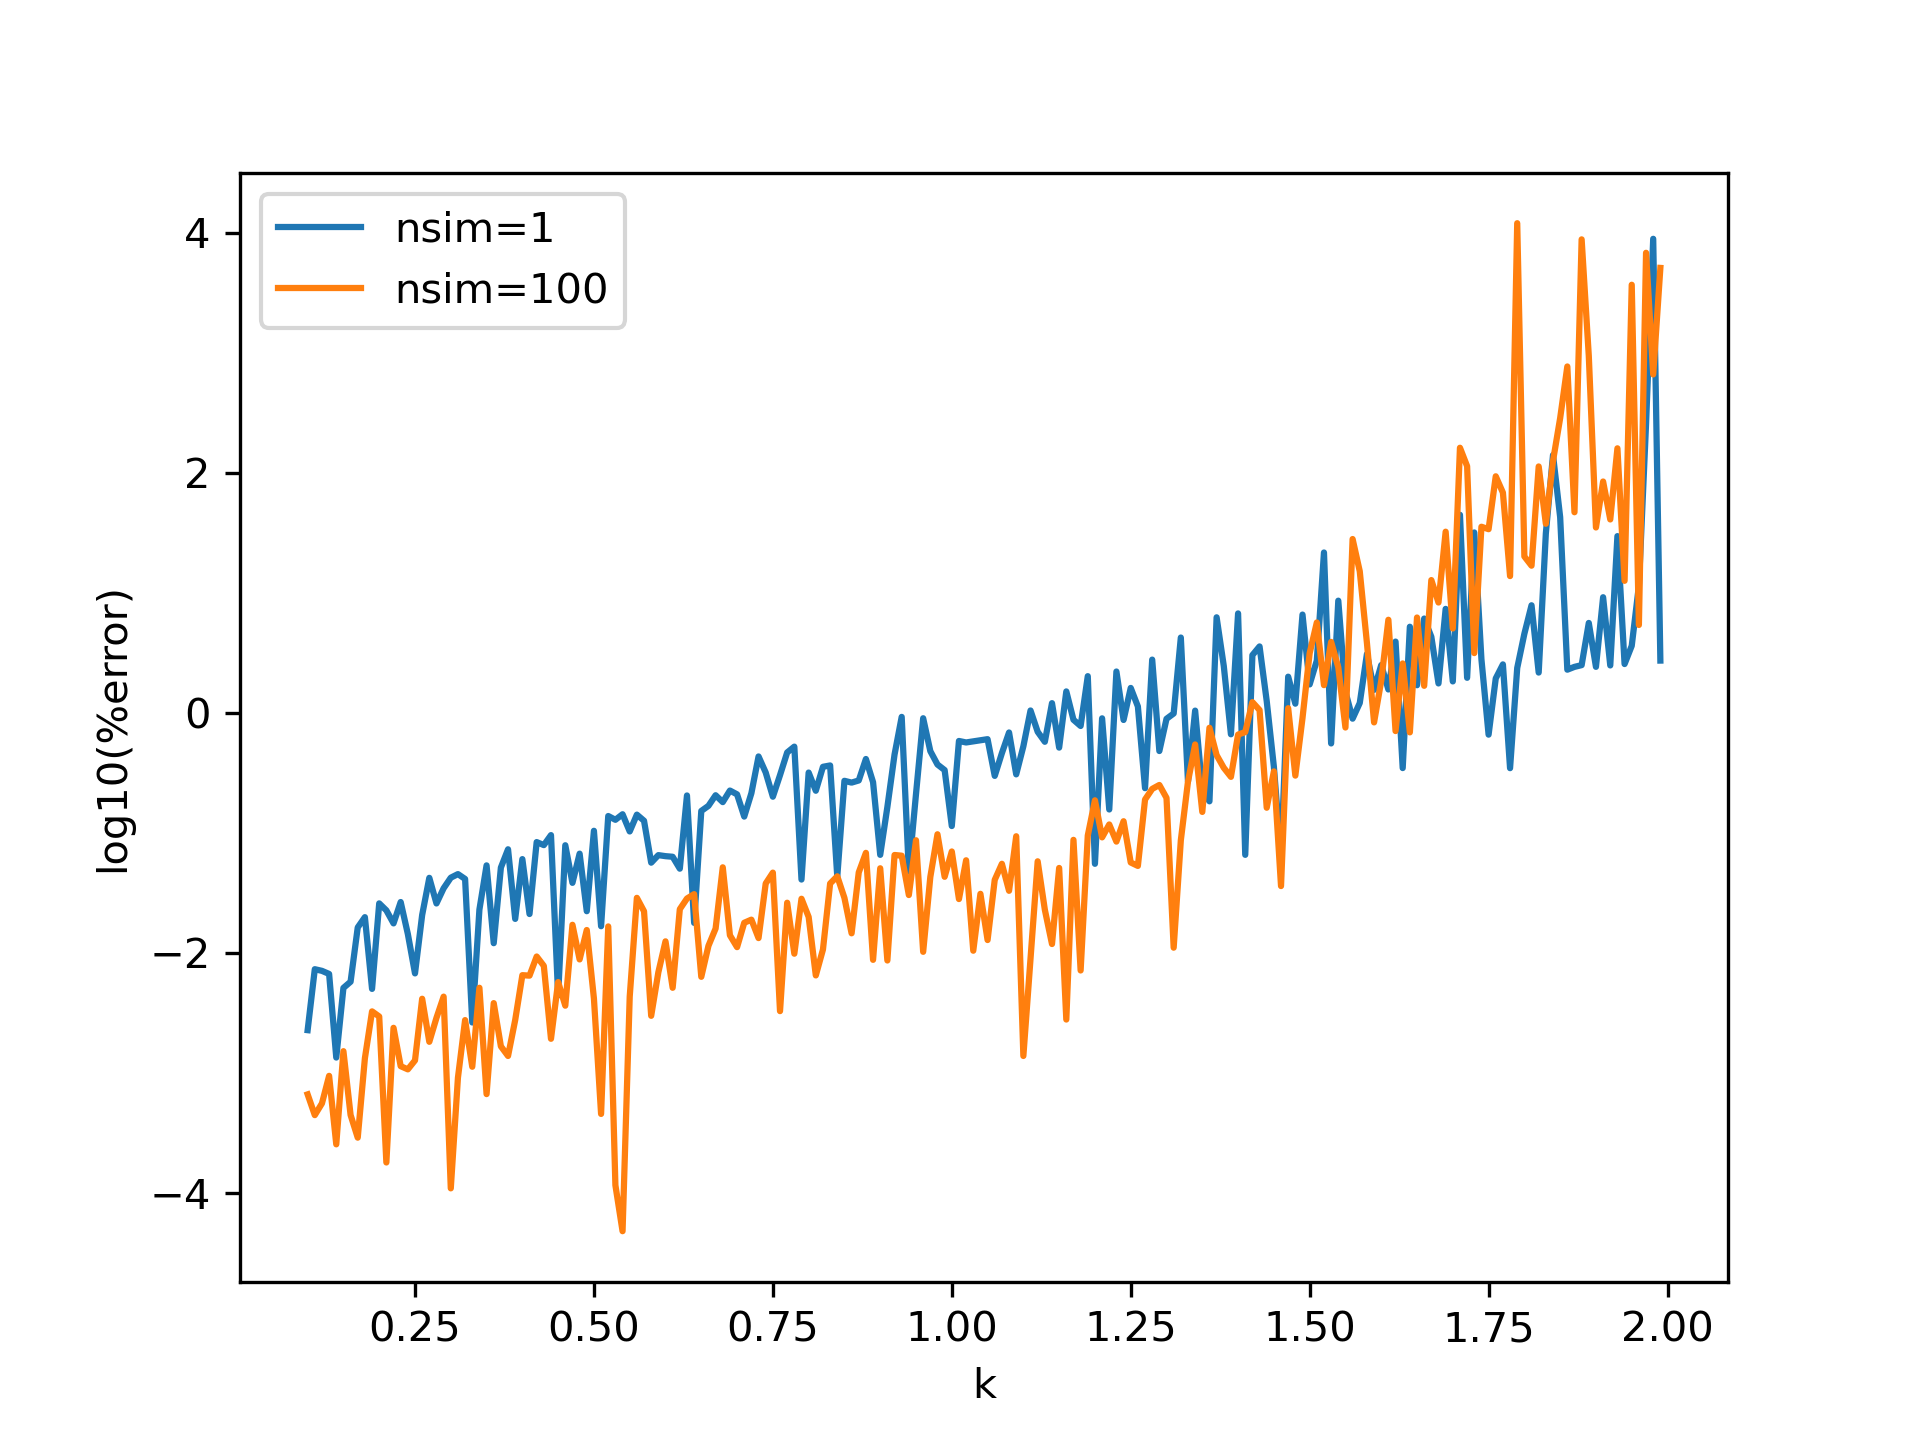
\includegraphics[width=0.8\textwidth]{plots/mainD explosion.png}
    \caption{The logarithmic percentage error of $Y(0)$ for
    (\ref{RRVE:main dirichlet}), with $l=1.2$ and initial conditions
    $y(-k)=e^{-k}$ and $y(k)=e^{k}$, displays an exponential
    increase until approximately $k=1.5$, beyond which additional
    simulations fail to reduce the error, indicating that the variance
    doesn't exist.}
    \label{fig:mainD explosion}
\end{figure}



\subsection{Initial Value Problems}
Classic IVP solvers rely on shrinking the time steps for
convergence. In this subsection we build up to
Recursion in Recursion MC (RRMC) for IVPs that tries to emulate
this behavior.


\begin{example}[RRMC $y'=y$] \label{ex:RRMC IVP}
    We demonstrate RRMC for IVPs with

    \begin{equation}
        y' = y, \quad y(0) = 1.
    \end{equation}

    Imagine we have a time-stepping scheme $(t_{n}), \forall n: t_{n-1} < t_{n}$
    then the following integral equations hold:

    \begin{equation}
        y(t)= y(t_{n}) + \int_{t_{n}}^{t}y(s)ds , \quad t>t_{n}.
    \end{equation}

    Turn these in the following class of RRVEs:

    \begin{equation}
        Y_{n}(t) = y(t_{n}) + (t-t_{n})Y_{n}((t-t_{n})U+t_{n}), \quad t>t_{n}.
    \end{equation}

    A problem with these RRVEs is that we do not know $y(t_{n})$.
    Instead, we can replace it with an unbiased estimate $y_{n}$
    which we keep frozen in the inner recursion:
    \begin{align}
        \label{eq:RRMC IVP inner}
        Y_{n}(t) & = y_{n} + (t-t_{n})Y_{n}((t-t_{n})U+t_{n}), \quad t>t_{n} \\
        y_{n}    & = \begin{cases}
                         Y_{n-1}(t_{n}) & \text{ if } n \neq 0 \\
                         y(t_{0})       & \text{ if } n = 0
                     \end{cases}.
        \label{eq:RRMC IVP outer}
    \end{align}
    We refer to equation (\ref{eq:RRMC IVP inner}) as the inner recursion and
    equation (\ref{eq:RRMC IVP outer}) as the outer recursion of the recursion in
    recursion.
\end{example}
% maybe measurements of amount of calls to f

\begin{pythonn}[implementation of (\ref{ex:RRMC IVP})] \label{py:RRMC IVP}
    \pythoncode{python code/RRMC_IVP.py}

    \begin{figure}[h!]
        \centering
        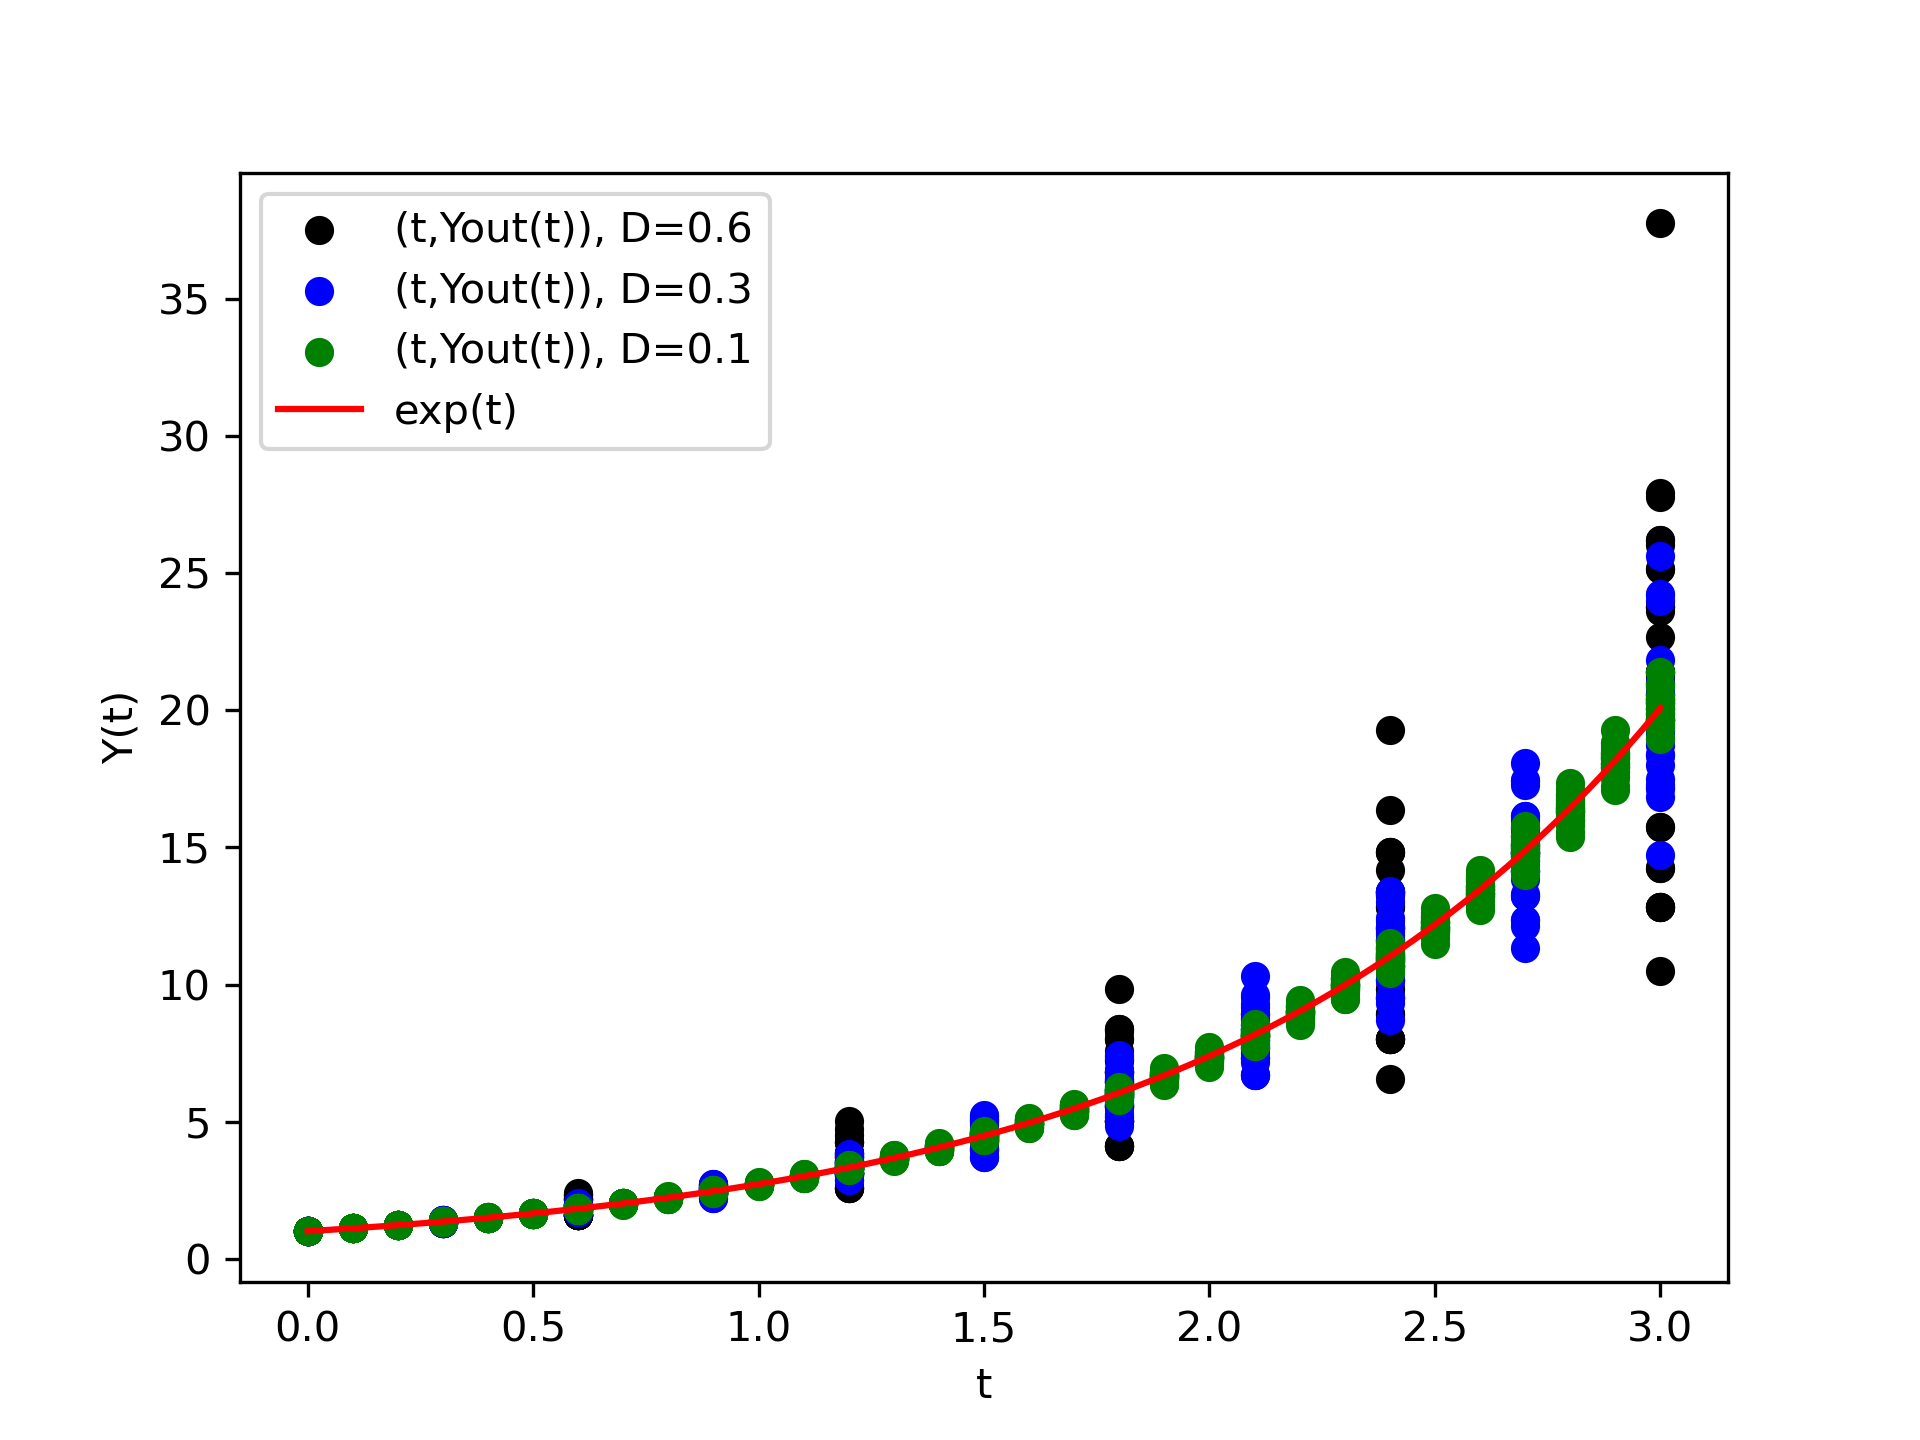
\includegraphics[width=0.8\textwidth]{plots/RRMC IVP.png}
        \caption{Recursive calls of equation (\ref{eq:RRMC IVP outer})
            when calling $Y_{\text{out}}(3,h)$ $30$ times for different $h$.  }
        \label{fig:RRMC IVP}
    \end{figure}
\end{pythonn}

We measured the convergence speed of example (\ref{ex:RRMC IVP}) to
be $O\left(\frac{h^{1.5}}{\sqrt{\text{nsim}}} \right)$.
While a $1.5$ order of convergence is commendable for an unbiased method,
it raises the question of how to attain even higher convergence orders.
It is possible to emulate classical methods to
achieve a higher order of convergence. This can be accomplished by eliminating
lower order terms by using control variates, as demonstrated in the MC trapezoidal
rule (see \ref{MCtrap}).

\begin{example}[CV RRMC $y'=y$]\label{ex:CV RRMC IVP}
    Let us control variate example (\ref{ex:RRMC IVP}).

    \begin{equation}
        y(t)= y(t_{n}) + \int_{t_{n}}^{t}y(s)ds , \quad t>t_{n}.
    \end{equation}

    We build a control variate with a lower-order approximation
    of the integrand:

    \begin{align}
        y(s) & = y(t_{n}) + (s-t_{n})y'(t_{n}) + O((s-t_{n})^{2})       \\
             & \approx y(t_{n}) + (s-t_{n})f(y(t_{n}),t_{n})            \\
             & \approx y(t_{n}) +
        (s-t_{n})\left(\frac{y(t_{n})-y(t_{n-1})}{t_{n}-t_{n-1}}\right) \\
             & \approx y(t_{n})(1+s-t_{n}).
    \end{align}

    Using the last one as a control variate for the integral:

    \begin{align}
        y(t) & = y(t_{n}) + \int_{t_{n}}^{t}y(s)ds                                          \\
             & = y(t_{n}) + \int_{t_{n}}^{t}y(s)-y(t_{n})(1+s-t_{n}) +y(t_{n})(1+s-t_{n})ds \\
             & = y(t_{n})\left(1 + (1-t_{n})(t-t_{n})+\frac{t^{2}-t_{n}^{2}}{2}\right)
        + \int_{t_{n}}^{t}y(s)-y(t_{n})(1+s-t_{n})ds.
    \end{align}

    We will not discuss turning this into an RRVE nor the implementation.
    The implementation is very similar to (\ref{py:nonlinear RRMC IVP}) and
    Figure \ref{fig:CV RRMC IVP} is a convergence plot for this example.

    \begin{figure}[h!]
        \centering
        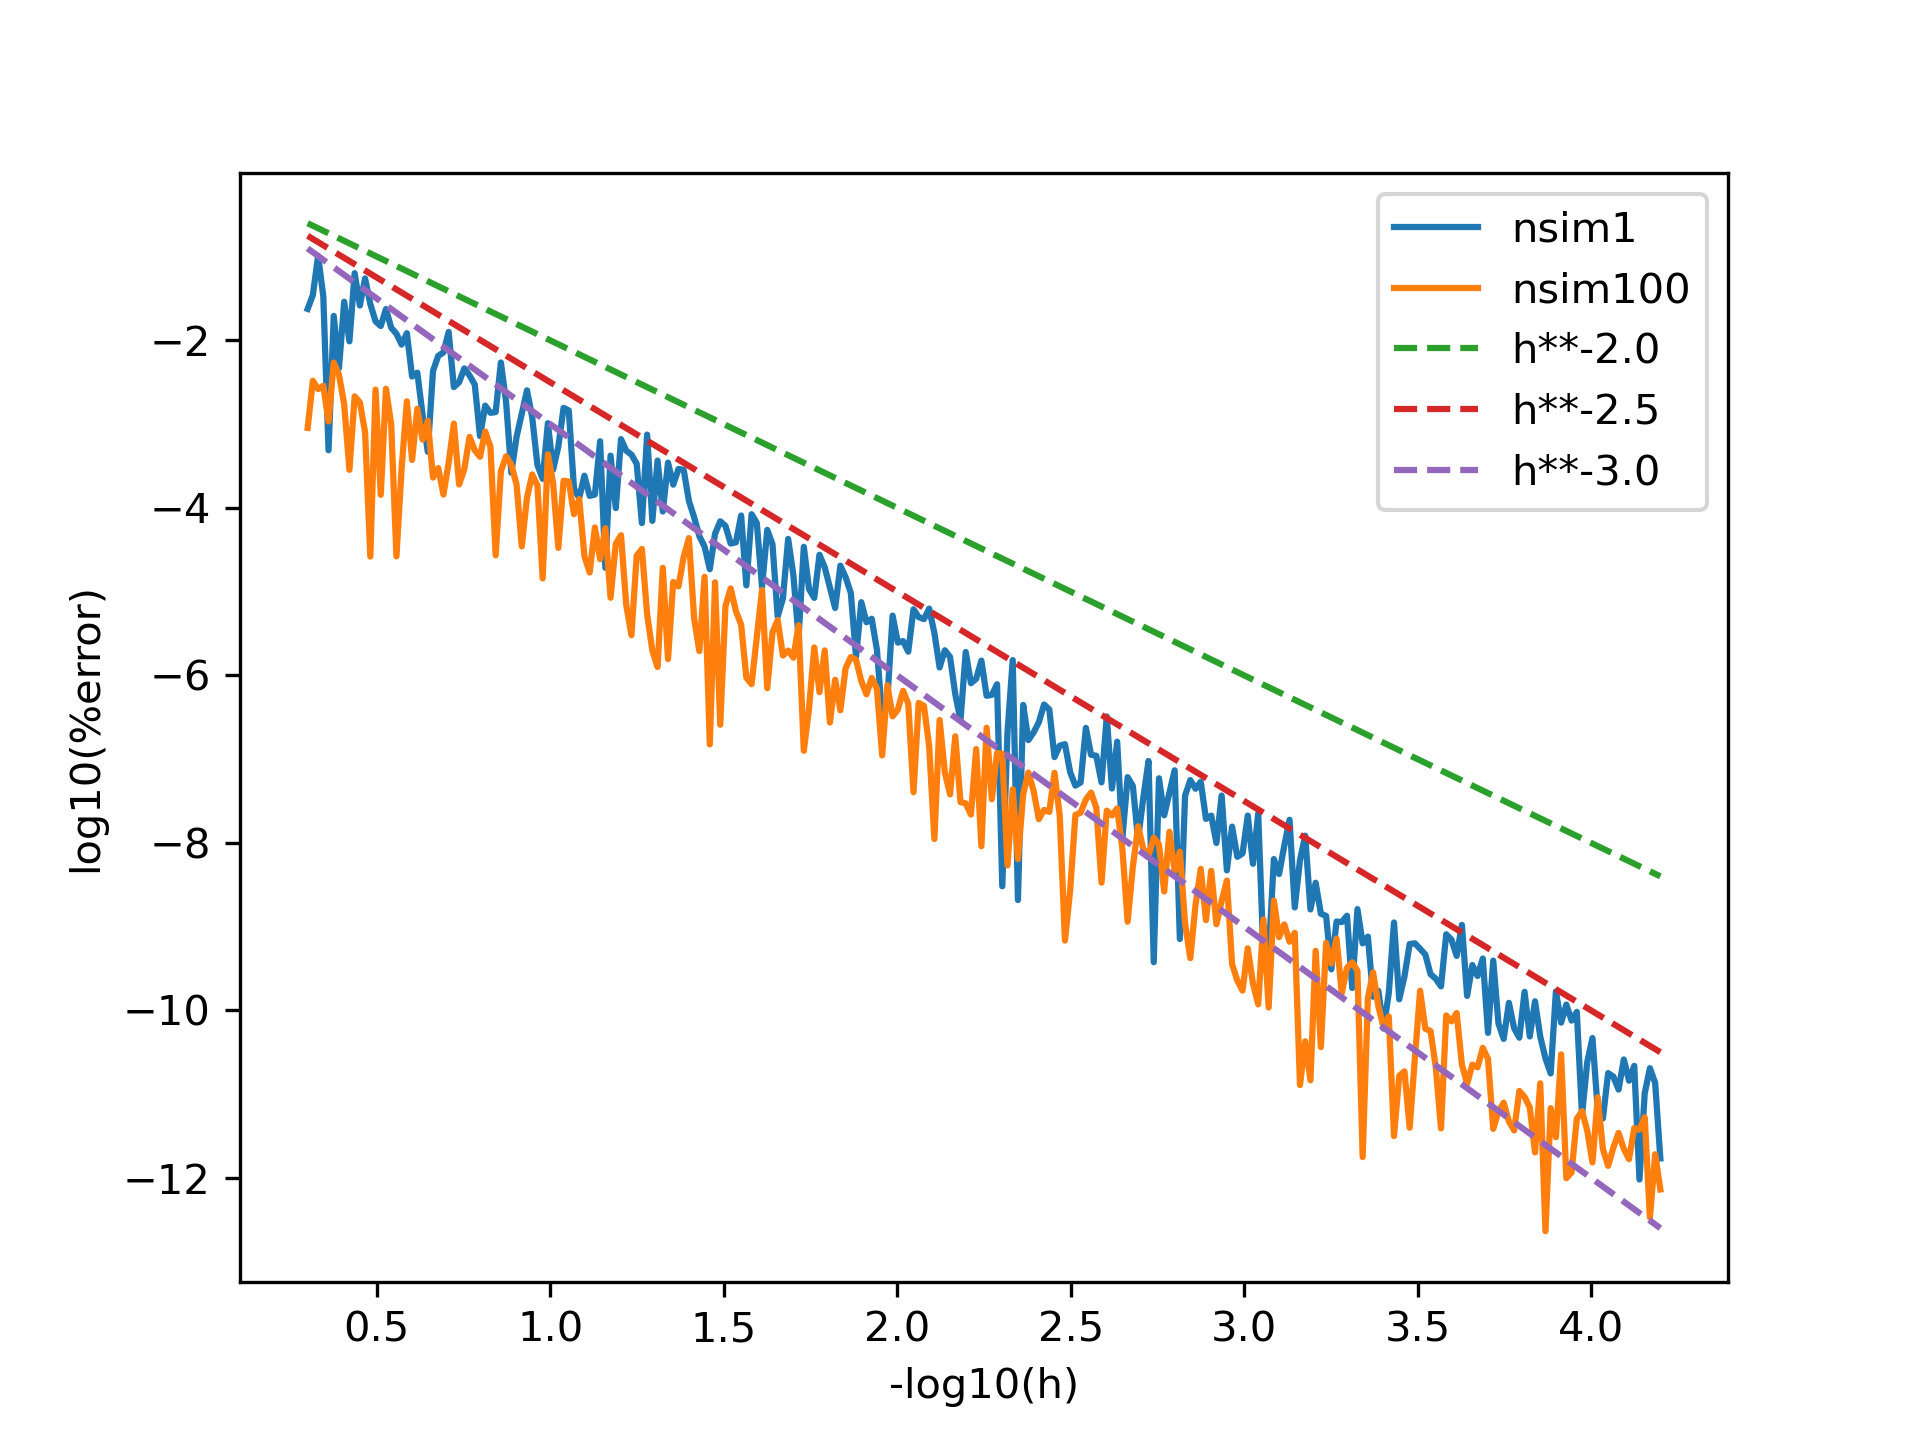
\includegraphics[width=0.8\textwidth]{plots/CV RRMC IVP.png}
        \caption{Log-log plot of the error for example
            (\ref{ex:CV RRMC IVP}) at $Y(10)$.}
        \label{fig:CV RRMC IVP}
    \end{figure}
\end{example}

\begin{related}[CV RRMC]
    \cite{daun_randomized_2011} similarly uses control variates to achieve
    a higher order of convergence.
\end{related}

RRMC is biased for our approach to non-linear problems.
The inner recursions are correlated because they use the same
information from the outer recursions, this does not mean that reducing
root-mean-square error by splitting does not work, you just have to be careful
with the bias. We conjecture that the bias in RRMC converges faster than the
variance when decreasing $h$.


\begin{example}[nonlinear RRMC IVP] \label{ex:nonlinear RRMC IVP}
    Consider the following IVP:

    \begin{equation}
        y' = y^{2} - t^{4} + 2t, \quad y(0) = 0.
    \end{equation}

    The exact solution to this problem is given by $y(t) = t^{2}$.
    We can express the solution as an integral equation:

    \begin{equation}
        y(t) = y(t_{n}) + \int_{t_{n}}^{t} y^{2}(s) ds
        - \frac{t^{5}-t_{n}^{5}}{5} + (t^{2}-t_{n}^{2}).
    \end{equation}

    By control variating $y^2(s)$ up to the second order using Taylor expansion,
    we have:

    \begin{align}
        y^2(t) & \approx y^2(t_n) + 2(t-t_n)y(t_n)y'(t_n) + ((t-t_n)y'(t_n))^2 + O((t-t_n)^2) \\
               & \approx y^2(t_n) + 2(t-t_n)y(t_n)y'(t_n) + O((t-t_n)^2)
    \end{align}

    Integrating the control variate yields:

    \begin{align}
        \int_{t_{n}}^{t} & y^{2}(t_{n}) + 2(s-t_{n})y(t_{n})y'(t_{n}) ds \\
                         & = (t-t_{n})y^{2}(t_{n})+
        2\left(\frac{t^{2}-t_{n}^{2}}{2} -t_{n}(t-t_{n}) \right)y(t_{n})y'(t_{n}).
    \end{align}
    We implement this example in (\ref{py:nonlinear RRMC IVP}).
\end{example}

\begin{pythonn}[implementation of (\ref{ex:nonlinear RRMC IVP})] \label{py:nonlinear RRMC IVP}
    \pythoncode{python code/nonlinear_CVRRMC.py}
\end{pythonn}


\section{Limitations and Future Work}

We have not dedicated significant attention, if any at all, to
the convergence analysis of RMC methods
for Fredholm equations. Figure \ref{fig:mainD explosion} illustrates
that arbitrary RMC do not converge. \\

Similarly to classic methods, RRMC struggles with big negative coefficients in front
of the recursive parts which may appear in
stiff problems.
In addition to the challenges with stiff problems, we have not conducted
a comparison between RRMC and traditional methods, and we do not anticipate
that RRMC in this form outperforms other classic methods.
The reason for this is that RRMC involves
many function calls in the inner recursion without updating the current control
variate. Proper testing requires precise tuning of the MC techniques utilized.
We do believe that RRMC could potentially offer advantages in atypical scenarios.
In the following example, we examine an ODE with a random parameter.

\begin{example}[random ODEs] \label{ex:random ode}
    Consider the problem given by the initial value problem
    \begin{equation}\label{eq:random ode}
        Y' = AY, \quad Y(0)=1, \quad A \sim \text{Uniform}(0,1).
    \end{equation}
    The solution to this problem is given by
    $Y(t) = e^{tA}$, which is a RV.
    In order to compute expectations of functions of $Y(t)$,
    we use unbiased estimates $X$ of the simulations of the solution.

    Given an analytic function $f$, we can obtain $E[f(Y(t))]$
    by conditioning on the value of $A$ and using the
    law of total expectation:
    \begin{align}
        E_A[f(Y(t))] & = E_A[f(Y(t)) \mid A]         \\
                     & = E_A[f(E_X[X(t,A)]) \mid A].
    \end{align}

    To estimate $f(E_X[X(t,A)])$, we use the approach outlined in
    (\ref{ex:exp int}). For the specific example of (\ref{eq:random ode}),
    we can compute the first two moments of $Y(t)$ as
    \begin{align}
        E_A[Y(t)]   & = \frac{e^t}{t} - \frac{1}{t},      \\
        E_A[Y^2(t)] & = \frac{e^{2t}}{2t} - \frac{1}{2t}.
    \end{align}
\end{example}

\begin{pythonn}[implementation of (\ref{ex:random ode})]
    \pythoncode{python code/random_ODE.py}
\end{pythonn}

\subsection{Heat Equation}
In this subsection, we introduce the relation between the heat equation and
Brownian motion.

\begin{definition}[$1$D heat equation Dirichlet] \label{def:heat equation}
    We define the $1$D heat equation for $u$ on connected domain $\Omega$
    with  Dirichlet boundary conditions the following way:
    \begin{equation}
        \frac{\partial u}{\partial t} = \frac{\partial^{2} u}{\partial x ^{2}}.
    \end{equation}
    Given $u(x,t)=\psi(x,t) ,\forall (x,t) \in \partial \Omega: t<\sup \{
        t| (x,t) \in \Omega\}$ .
\end{definition}

\begin{lemma}[Brownian motion and the heat equation] \label{lem:BM HE}
    For problem (\ref{def:heat equation}) if $ |\psi|$ is bounded
    then there holds:

    \begin{equation}
        u(x,t)=E[\psi(Y_{\tau},\tau) | Y_{t} =x].
    \end{equation}
    With $dY_{s} = dW_{-s},\tau = \sup\{s | (Y_{s},s) \notin \Omega\}$.
\end{lemma}


\begin{proof} \label{proof: BM HE }
    Discretize the heat equation
    with a regular rectangular mesh that includes $(x,t)$ with equally
    spaced intervals over space and time ($\Delta x, \Delta t$) with
    the corresponding difference equation:

    \begin{equation}
        \frac{u(x,t)-u(x,t-\Delta t)}{\Delta t} = \frac{u(x + \Delta x,t)-2 u(x,t) +u(x - \Delta x,t)}{\Delta x^{2}} .
    \end{equation}

    Isolate $u(x,t)$:

    \begin{equation} \label{eq:discrete iso heat equation}
        u(x,t) =
        \frac{\Delta t}{ 2 \Delta t + \Delta x^{2}}
        \left(
        u(x+\Delta x,t)+u(x-\Delta x,t)
        \right) +
        \frac{\Delta x^{2}}{ 2 \Delta t + \Delta x^{2}}
        \left(
        u(x,t-\Delta t)
        \right).
    \end{equation}

    Because $u(x+\Delta x,t) \approx u(x-\Delta x,t) \approx u(x,t-\Delta t) \approx$
    right-hand side of equation (\ref{eq:discrete iso heat equation}) we may Russian roulette
    to remove branching recursion and generate a recursion path instead of a tree.
    \begin{equation} \label{eq:RRVE discrete heat equation }
        Z(x,t) =
        \begin{cases}
            \psi(\text{argmin}_{b \in \partial \Omega} ||(x,t) - b||)
             & \text{ when } (x,t) \notin \Omega \\
            \begin{cases}
                Z(x+\Delta x , t)  & \text{ with chance  } \frac{\Delta t}{ 2 \Delta t + \Delta x^{2}}     \\
                Z(x-\Delta x , t)  & \text{ with chance  } \frac{\Delta t}{ 2 \Delta t + \Delta x^{2}}     \\
                Z(x, t - \Delta t) & \text{ with chance  } \frac{\Delta x^{2}}{ 2 \Delta t + \Delta x^{2}}
            \end{cases}
             & \text{ else }.
        \end{cases}
    \end{equation}
    This is a RRVE, $Z$ has finite variance because $ |\psi|$ is bounded
    and $E[Z(x,t)]$ is the solution to the discretized heat equation. Taking the limit
    makes the discrete solution converge to the real solution.
    For (\ref{eq:RRVE discrete heat equation }) the limit
    makes the recursion path go to Brownian motion $Y_{t}$.
    \begin{equation}
        Z(x,t) \rightarrow \psi(Y_{\tau},\tau)  .
    \end{equation}
    Finishing the proof.
\end{proof}

\begin{related}
    (\ref{lem:BM HE}) is a subcase of the Feynman-Kac formula.
    For a proof and an in-depth discussion of the Feynman-Kac formula
    see \cite{oksendal_stochastic_2003}. \\
\end{related}


\newpage
\begin{abstract}
    Deze scriptie onderzoekt unbiased Monte Carlo methoden voor
het oplossen van lineaire gewone differentiaalvergelijkingen met het
oog op partiële differentiaalvergelijkingen.
De voorgestelde algoritmes maken gebruik van de geschikte
combinatie van Monte Carlo technieken. Deze Monte Carlo technieken
worden geïntroduceerd met voorbeelden en code.
\end{abstract}

\printbibliography
\newpage

\end{document}

% Base your answers on the thesis.  
% You are expert in solving ODEs, WoS, IBC, PDEs giving feedback.
%
% Answer as a markdown file.
% Use subnumerings in mark down form in numbering the question 
% that works in a markdown file and use different headers. Like this: 
%
% # Content tests
% ##  0.1. How does the main algorithm work of the thesis?
% answer
%
% Here are the questions : 
% # Content tests
% 0.1. How does the main algorithm work of the thesis?
% 0.2. What is the biggest limitation of the main algorithm of the thesis?
% 0.3. How important is coupled splitting to the thesis?
% 0.4. How does Stein's paradox pop up in the thesis? (see subsection on MC integration)
% 0.5. Rate the language of the thesis.
% 0.6. List the 5 unclearest parts of the thesis.
% 0.7. What is special about the Monte Carlo trapezoidal rule?
% 0.8. What is the main advantage of the primary motivating work? 
% 0.9.  How does the thesis define Russian Roulette?
% 0.10. How does the thesis define control variates?
% 0.11. Summarize the approach for exponential of the expectance in the unbiased non-linearity section.
% 0.12. How does the thesis define tail recursion?
% 0.13. How does the thesis define Green's functions? 
% 0.14. Summarize convergence behavior of the main algorithm.
% 0.15. List your 5 favorite/intrestring parts of the thesis.
% 0.16. What seem to be missing in the thesis?
% 0.17. Any abbreviation that should/shouldn't be used?
% 0.18. List 5 inaccuracies things in the thesis.
% 0.19. List 5 controversial things in the thesis.
% 0.20. List 5 suggestions to improve the thesis.
%
% # Feedback 1
% 1.1 Does the thesis differentiate between the original contributions and prior work? 
% 1.2 Does the thesis has a good overview?
% 1.3 Does the thesis has a good conclusion?
% 1.4 Does everything gets defined in the thesis?
% 1.5 Are there symbols that don't get defined in the thesis?
% 1.6 What are the advantages of the solvers in the subsection of initial value problems 
% compared to classical solver?
% 1.7 Are the explanations for the graphs in the thesis sufficient?
% 1.8 Do equations, examples, definition, etc get referenced with consistent notation?
% 1.9 List 2 uncommon abbreviations that don't get introduced the first time they get used. 
%
% # Feedback 2
% 2.1 Has the elementary theory of Monte Carlo been covered in the thesis?
% 2.2 In the subsection of recursive Monte Carlo why is there indefinite 
% recursion?
% 2.3 Does the thesis give the necessary references to concepts?
% 2.4 Does additive branching gets explained clearly?
% 2.5 What is the Russian roulette rate ?
% 2.6 Does the local truncation error get defined ?

% # Requirements
% 3.1 Title Page: Does the thesis have a title page? 
% 3.2 Table of Contents: Does the thesis include a table of contents?
% 3.3 Introduction: 
%     Does the introduction provide a clear context for the research?
%     Is the problem statement or research question clearly formulated in the introduction?

% 3.4 Exposition:
%     Is the argumentation detailed and logical, leading to the final result of the research?
%     Is the substructure effectively used to organize and clarify the content within the exposition?

% 3.5 Dutch Summary:

%     Does the thesis include a Dutch summary?
%     Is the Dutch summary concise, effectively summarizing the main points of the thesis within the specified page limit?

% 3.6 Bibliography:

%     Is the bibliography section present and well-structured?
%     Are all the cited sources accurately listed in the bibliography according to the specified citation style?

% 3.7 Layout and Readability:
%   - Is the layout designed to enhance readability, including appropriate font, line spacing, and paragraph structure?
%   -  Is the use of headings, subheadings, and other formatting elements consistent and effective in guiding the reader through the content?

% 3.8 Language Quality:
% - Is the language used throughout the thesis refined and well-crafted?
% - Are grammar, spelling, and punctuation accurate?

% 3.9 Results and Analysis:

% - Are the results presented clearly and comprehensively?
% - Is the analysis of the results thorough, and do the conclusions logically follow from the data?

% 3.10 Argumentation and Coherence:

% - Is there a clear and logical progression of ideas throughout the thesis?
% - Do transitions between sections and paragraphs enhance the overall coherence of the document?

% 3.11 Original Contribution:
% - Does the thesis make a unique and valuable contribution to the field of study?
% - Is there a clear statement about how the research fills a gap in existing knowledge?

% 3.12 Discussion and Implications:
% - Does the discussion section provide insights into the broader implications of the research findings?
% - Are any practical applications or future research directions suggested?

% 3.13 Clarity and Conciseness:
% - Is the writing style clear and concise, avoiding unnecessary jargon?
% - Are complex concepts explained in a way that is understandable to the intended audience?

% 3.14 Overall Contribution:
% - Does the thesis contribute significantly to the field's body of knowledge and understanding?
% - Is the thesis likely to be cited and referenced by others in the field?

